\chapter{Mathematical Background}\label{0-Mathematical-Backgroun}

This is a brief review of some mathematical tools, and especially
probability theory, that we will use in this course. See also the
\href{http://www.introtcs.org/public/lec_00_1_math_background.html}{mathematical
background} and
\href{http://www.introtcs.org/public/lec_15_probability.html}{probability}
lectures in my \href{http://www.introtcs.org/}{Notes on Introduction to
Theoretical Computer Science}, which share much of the following text.

At Harvard, much of this material (and more) is taught in Stat 110
``Introduction to Probability'', CS20 ``Discrete Mathematics'', and
AM107 ``Graph Theory and Combinatorics''. Some good sources for this
material are the lecture notes by Papadimitriou and Vazirani (see home
page of Umesh Vaziarani), Lehman, Leighton and Meyer from MIT Course
6.042 ``Mathematics For Computer Science'' (Chapters 1-2 and 14 to 19
are particularly relevant), and the Berkeley course CS 70. The
mathematical tool we use most often is discrete probability. The
``Probabilistic Method'' book by Alon and Spencer is a great resource in
this area. Also, the books of Mitzenmacher and Upfal and Prabhakar and
Raghavan cover probability from a more algorithmic perspective. For an
excellent popular discussion of some of the mathematical concepts we'll
talk about see the book \emph{``How Not to Be Wrong''} by Jordan
Ellenberg.

Although knowledge of algorithms is not strictly necessary, it would be
quite useful. Students who did not take an algorithms class such as CS
124 might want to look at one of the books (1) Corman, Leiserson, Rivest
and Smith, (2) Dasgupte, Papadimitriou and Vaziarni, or (3) Kleinberg
and Tardos. We do not require prior knowledge of complexity or
computability but some basic familiarity could be useful. Students who
did not take a theory of computation class such as CS 121 might want to
look at my lecture notes or the first 2 chapters of my book with Arora.

\section{A quick overview of mathematical
prerequisites}\label{0-A-quick-overview-of-ma}

The main notions we will use in this course are the following:

\begin{itemize}
\item
  \textbf{Proofs:} First and foremost, this course will involve a heavy
  dose of formal mathematical reasoning, which includes mathematical
  \emph{definitions}, \emph{statements}, and \emph{proofs}.
\item
  \textbf{Sets and functions:} We will assume familiarity with basic
  notions of sets and operations on sets such as union (denoted
  \(\cup\)), intersection (denoted \(\cap\)), and set substraction
  (denoted \(\setminus\)). We denote by \(|A|\) the size of the set
  \(A\). We also assume familiarity with functions, and notions such as
  one-to-one (injective) functions and onto (surjective) functions. If
  \(f\) is a function from a set \(A\) to a set \(B\), we denote this by
  \(f:A\rightarrow B\). If \(f\) is one-to-one then this implies that
  \(|A| \leq |B|\). If \(f\) is onto then \(|A| \geq |B|\). If \(f\) is
  a permutation/bijection (e.g., one-to-one \emph{and} onto) then this
  implies that \(|A|=|B|\).
\item
  \textbf{Big Oh notation:} If \(f,g\) are two functions from
  \({\mathbb{N}}\) to \({\mathbb{N}}\), then (1) \(f = O(g)\) if there
  exists a constant \(c\) such that \(f(n) \leq c\cdot g(n)\) for every
  sufficiently large \(n\), (2) \(f = \Omega(g)\) if \(g=O(f)\), (3)
  \(f = \Theta(g)\) is \(f=O(g)\) and \(g=O(f)\), (4) \(f = o(g)\) if
  for every \(\epsilon>0\), \(f(n) \leq \epsilon \cdot g(n)\) for every
  sufficiently large \(n\), and (5) \(f = \omega(g)\) if \(g = o(f)\).
  To emphasize the input parameter, we often write \(f(n) = O(g(n))\)
  instead of \(f = O(g)\), and use similar notation for
  \(o,\Omega,\omega,\Theta\). While this is only an imprecise heuristic,
  when you see a statement of the form \(f(n)=O(g(n))\) you can often
  replace it in your mind by the statement \(f(n) \leq 1000g(n)\) while
  the statement \(f(n) = \Omega(g(n))\) can often be thought of as
  \(f(n)\geq 0.001g(n)\) .
\item
  \textbf{Logical operations:} The operations AND, OR, and NOT
  (\(\wedge,\vee,\neg\)) and the quantifiers ``exists'' and ``forall''
  (\(\exists\),\(\forall\)).
\item
  \textbf{Tuples and strings:} The notation \(\Sigma^k\) and
  \(\Sigma^*\) where \(\Sigma\) is some finite set which is called the
  \emph{alphabet} (quite often \(\Sigma = \{0,1\}\)).
\item
  \textbf{Graphs:} Undirected and directed graphs, connectivity, paths,
  and cycles.
\item
  \textbf{Basic combinatorics:} Notions such as \(\binom{n}{k}\) (the
  number of \(k\)-sized subset of a set of size \(n\)).
\item
  \textbf{Discrete probability:} We will extensively use
  \emph{probability theory}, and specifically probability over
  \emph{finite} samples spaces such as tossing \(n\) coins, including
  notions such as \emph{random variables}, \emph{expectation}, and
  \emph{concentration}.
\item
  \textbf{Modular arithmetic:} We will use
  \href{https://en.wikipedia.org/wiki/Modular_arithmetic}{modular
  arithmetic} (i.e., addition and multiplication modulo some number
  \(m\)), and in particular talk about operations on vectors and
  matrices whose elements are taken modulo \(m\). If \(n\) is an
  integer, then we denote by \(a \pmod{n}\) the remainder of \(a\) when
  divided by \(n\). \(a\pmod{n}\) is the number \(r\in\{0,\ldots,n-1\}\)
  such that \(a = kn+r\) for some integer \(k\). It will be very useful
  that \(a\pmod{n} + b \pmod{n} = (a+b) \pmod{n}\) and
  \(a\pmod{n} \cdot b \pmod{n} = (a\cdot b) \pmod{n}\) and so modular
  arithmetic inherits all of the rules (associativity, commutativity
  etc..) of integer arithmetic. If \(a,b\) are positive integers then
  \(gcd(a,b)\) is the largest integer that divides both \(a\) and \(b\).
  It is known that for every \(a,b\) there exist (not necessarily
  positive) integers \(x,y\) such that \(ax + by = gcd(a,b)\) (it's a
  good exercise to prove this on your own). In particular, if
  \(gcd(a,n)=1\) then there exists a \emph{modular inverse} for \(a\)
  which is a number \(b\) such that \(ab = 1 \pmod{n}\). We sometimes
  write \(b\) as \(a^{-1} \pmod{n}\).
\item
  \textbf{Group theory, linear algebra:} In later parts of the course we
  will need the notions of matrices, vectors, matrix multiplication and
  inverse, determinant, eigenvalues, and eigenvectors. These can be
  picked up in any basic text on linear algebra. In some parts we might
  also use some basic facts of group theory (finite groups only, and
  mostly only commutative ones). These also can be picked up as we go
  along, and a prior course on group theory is not necessary.
\item
  \textbf{Discrete probability:} \emph{Probability theory}, and
  specifically probability over \emph{finite} samples spaces such as
  tossing \(n\) coins is a crucial part of cryptography, since (as we'll
  see) there is no secrecy without randomness.
\end{itemize}

~

\section{Mathematical Proofs}\label{0-Mathematical-Proofs}

Arguably \emph{the} mathematical prerequisite needed for this course is
a certain level of comfort with mathematical proofs. Many students tend
to think of mathematical proofs as a very formal object, like the proofs
studied in school in geometry, consisting of a sequence of axioms and
statements derived from them by very specific rules. In fact,

\begin{quote}
\emph{a proof is a piece of writing meant to convince human readers that
a particular statement is true.}
\end{quote}

(In this class, the particular humans you are trying to convince are me
and the teaching fellows.)

To write a proof of some statement X you need to follow three steps:

\begin{enumerate}
\def\labelenumi{\arabic{enumi}.}
\item
  Make sure that you completely understand the statement X.
\item
  Think about X until you are able to convince \emph{yourself} that X is
  true.
\item
  Think how to present the argument in the clearest possible way so you
  can convince the reader as well.
\end{enumerate}

Like any good piece of writing, a proof should be concise and not be
overly formal or cumbersome. In fact, overuse of formalism can often be
\emph{detrimental} to the argument since it can mask weaknesses in the
argument from both the writer and the reader. Sometimes students try to
``throw the kitchen sink'' at an answer trying to list all possibly
relevant facts in the hope of getting partial credit. But a proof is a
piece of writing, and a badly written proof will not get credit even if
it contains some correct elements. It is better to write a clear proof
of a partial statement. In particular, if you haven't been able to
convince yourself that the statement is true, you should be honest about
it and explain which parts of the statement you have been able to verify
and which parts you haven't.

\subsection{Example: The existence of infinitely many
primes.}\label{0-Example-The-existence-}

In the spirit of ``do what I say and not what I do'', I will now
demonstrate the importance of conciseness by belaboring the point and
spending several paragraphs on a simple proof, written by Euclid around
300 BC. Recall that a \emph{prime number} is an integer \(p>1\) whose
only divisors are \(p\) and \(1\). Euclid's Theorem is the following:

\hypertarget{infprimesthm}{}
\begin{theorem}[Infinitude of primes] \label[theorem]{infprimesthm}

There exist infinitely many primes.

\end{theorem}

Instead of simply writing down the proof, let us try to understand how
we might figure this proof out. (If you haven't seen this proof before,
or you don't remember it, you might want to stop reading at this point
and try to come up with it on your own before continuing.) The first
(and often most important) step is to understand what the statement
means. Saying that the number of primes is infinite means that it is not
finite. More precisely, this means that for every natural number \(k\),
there are more than \(k\) primes.

Now that we understand what we need to prove, let us try to convince
ourselves of this fact. At first, it might seem obvious--- since there
are infinitely many natural numbers, and every one of them can be
factored into primes, there must be infinitely many primes, right?

Wrong. Since we can compose a prime many times with itself, a finite
number of primes can generate infinitely many numbers. Indeed the single
prime \(3\) generates the infinite set of all numbers of the form
\(3^n\). So, what we really need to show is that for every finite set of
primes \(\{ p_1,\ldots,p_k\}\), there exists a number \(n\) that has a
prime factor outside this set.

Now we need to start playing around. Suppose that we had just two primes
\(p\) and \(q\). How would we find a number \(n\) that is not generated
by \(p\) and \(q\)? If you try to draw things on the number line, you
would see that there is always some \emph{gap} between multiples of
\(p\) and \(q\) in the sense that they are never consecutive. It is
possible to prove that (in fact, it's not a bad exercise) but this
observation already suggests a guess for what would be a number that is
divisible by neither \(p\) nor \(q\), namely \(pq+1\). Indeed, the
remainder of \(n=pq+1\) when dividing by either \(p\) or \(q\) would be
\(1\) (which in particular is not zero). This observation generalizes
and we can set \(n=pqr+1\) to be a number that is divisible neither by
\(p,q\) nor \(r\), and more generally \(n=p_1\cdots, p_k +1\) is not
divisible by \(p_1,\ldots,p_k\).

Now we have convinced ourselves of the statement and it is time to think
of how to write this down in the clearest way. One issue that arises is
that we want to prove things truly from the definition of primes and
first principles, and so not assume properties of division and
remainders or even the existence of a prime factorization, without
proving it. Here is what a proof could look like. We will prove the
following two lemmas:

\hypertarget{primesfirstlem}{}
\begin{lemma}[Existence of prime divisor] \label[lemma]{primesfirstlem}

For every integer \(n>1\), there exists a prime \(p>1\) that divides
\(n\).

\end{lemma}

\hypertarget{primesseclem}{}
\begin{lemma}[Existence of co-prime] \label[lemma]{primesseclem}

For every set of integers \(p_1,\ldots,p_k>1\), there exists a number
\(n\) such that none of \(p_1,\ldots,p_k\) divide \(n\).

\end{lemma}

From these two lemmas it follows that there exist infinitely many
primes, since otherwise if we let \(p_1,\ldots,p_k\) be the set of all
primes, then we would get a contradiction as by combining
\cref{primesfirstlem} and \cref{primesseclem} we would get a number
\(n\) with a prime factor outside this set. We now prove the lemmas:

\begin{proof}[Proof of \cref{primesfirstlem}] \label[proof]{0-Let-n-be-a-number-and-}

Let \(n>1\) be a number, and let \(p\) be the smallest divisor of \(n\)
that is larger than \(1\) (there exists such a number \(p\) since \(n\)
divides itself). We claim that \(p\) is a prime. Indeed suppose
otherwise there was some \(1< q < p\) that divides \(p\). Then since
\(n = pc\) for some integer \(c\) and \(p=qc'\) for some integer \(c'\)
we'll get that \(n=qcc'\) and hence \(q\) divides \(n\) in contradiction
to the choice of \(p\) as the smallest divisor of \(n\).

\end{proof}

\begin{proof}[Proof of \cref{primesseclem}] \label[proof]{0-Let-np-cdots-pk---and-}

Let \(n=p_1 \cdots p_k + 1\) and suppose for the sake of contradiction
that there exists some \(i\) such that \(n = p_i\cdot c\) for some
integer \(c\). Then if we divide the equation \(n - p_1 \cdots p_k = 1\)
by \(p_i\) then we get \(c\) minus an integer on the lefthand side, and
the fraction \(1/p_i\) on the righthand side.

\end{proof}

This completes the proof of \cref{infprimesthm}

\section{Probability and Sample spaces}\label{0-Probability-and-Sample}

Perhaps the main mathematical background needed in cryptography is
probability theory since, as we will see, there is no secrecy without
randomness. Luckily, we only need fairly basic notions of probability
theory and in particular only probability over finite sample spaces. If
you have a good understanding of what happens when we toss \(k\) random
coins, then you know most of the probability you'll need. The discussion
below is not meant to replace a course on probability theory, and if you
have not seen this material before, I highly recommend you look at
additional resources to get up to speed.\footnote{Harvard's
  \href{http://projects.iq.harvard.edu/stat110/home}{STAT 110} class
  (whose lectures are available on
  \href{http://projects.iq.harvard.edu/stat110/youtube}{youtube} ) is a
  highly recommended introduction to probability. See also these
  \href{http://www.boazbarak.org/cs121/LLM_probability.pdf}{lecture
  notes} from MIT's ``Mathematics for Computer Science'' course ,as well
  as notes 12-17 of Berkeley's \href{https://www.eecs70.org/}{CS 70}.}

The nature of randomness and probability is a topic of great
philosophical, scientific and mathematical depth. Is there actual
randomness in the world, or does it proceed in a deterministic clockwork
fashion from some initial conditions set at the beginning of time? Does
probability refer to our uncertainty of beliefs, or to the frequency of
occurrences in repeated experiments? How can we define probability over
infinite sets?

These are all important questions that have been studied and debated by
scientists, mathematicians, statisticians and philosophers. Fortunately,
we will not need to deal directly with these questions here. We will be
mostly interested in the setting of tossing \(n\) random, unbiased and
independent coins. Below we define the basic probabilistic objects of
\emph{events} and \emph{random variables} when restricted to this
setting. These can be defined for much more general probabilistic
experiments or \emph{sample spaces}, and later on we will briefly
discuss how this can be done. However, the \(n\)-coin case is sufficient
for almost everything we'll need in this course.

If instead of ``heads'' and ``tails'' we encode the sides of each coin
by ``zero'' and ``one'', we can encode the result of tossing \(n\) coins
as a string in \(\{0,1\}^n\). Each particular outcome \(x\in \{0,1\}^n\)
is obtained with probability \(2^{-n}\). For example, if we toss three
coins, then we obtain each of the 8 outcomes
\(000,001,010,011,100,101,110,111\) with probability \(2^{-3}=1/8\) (see
also \cref{coinexperimentfig}). We can describe the experiment of
tossing \(n\) coins as choosing a string \(x\) uniformly at random from
\(\{0,1\}^n\), and hence we'll use the shorthand \(x\sim \{0,1\}^n\) for
\(x\) that is chosen according to this experiment.

\begin{marginfigure}
\centering
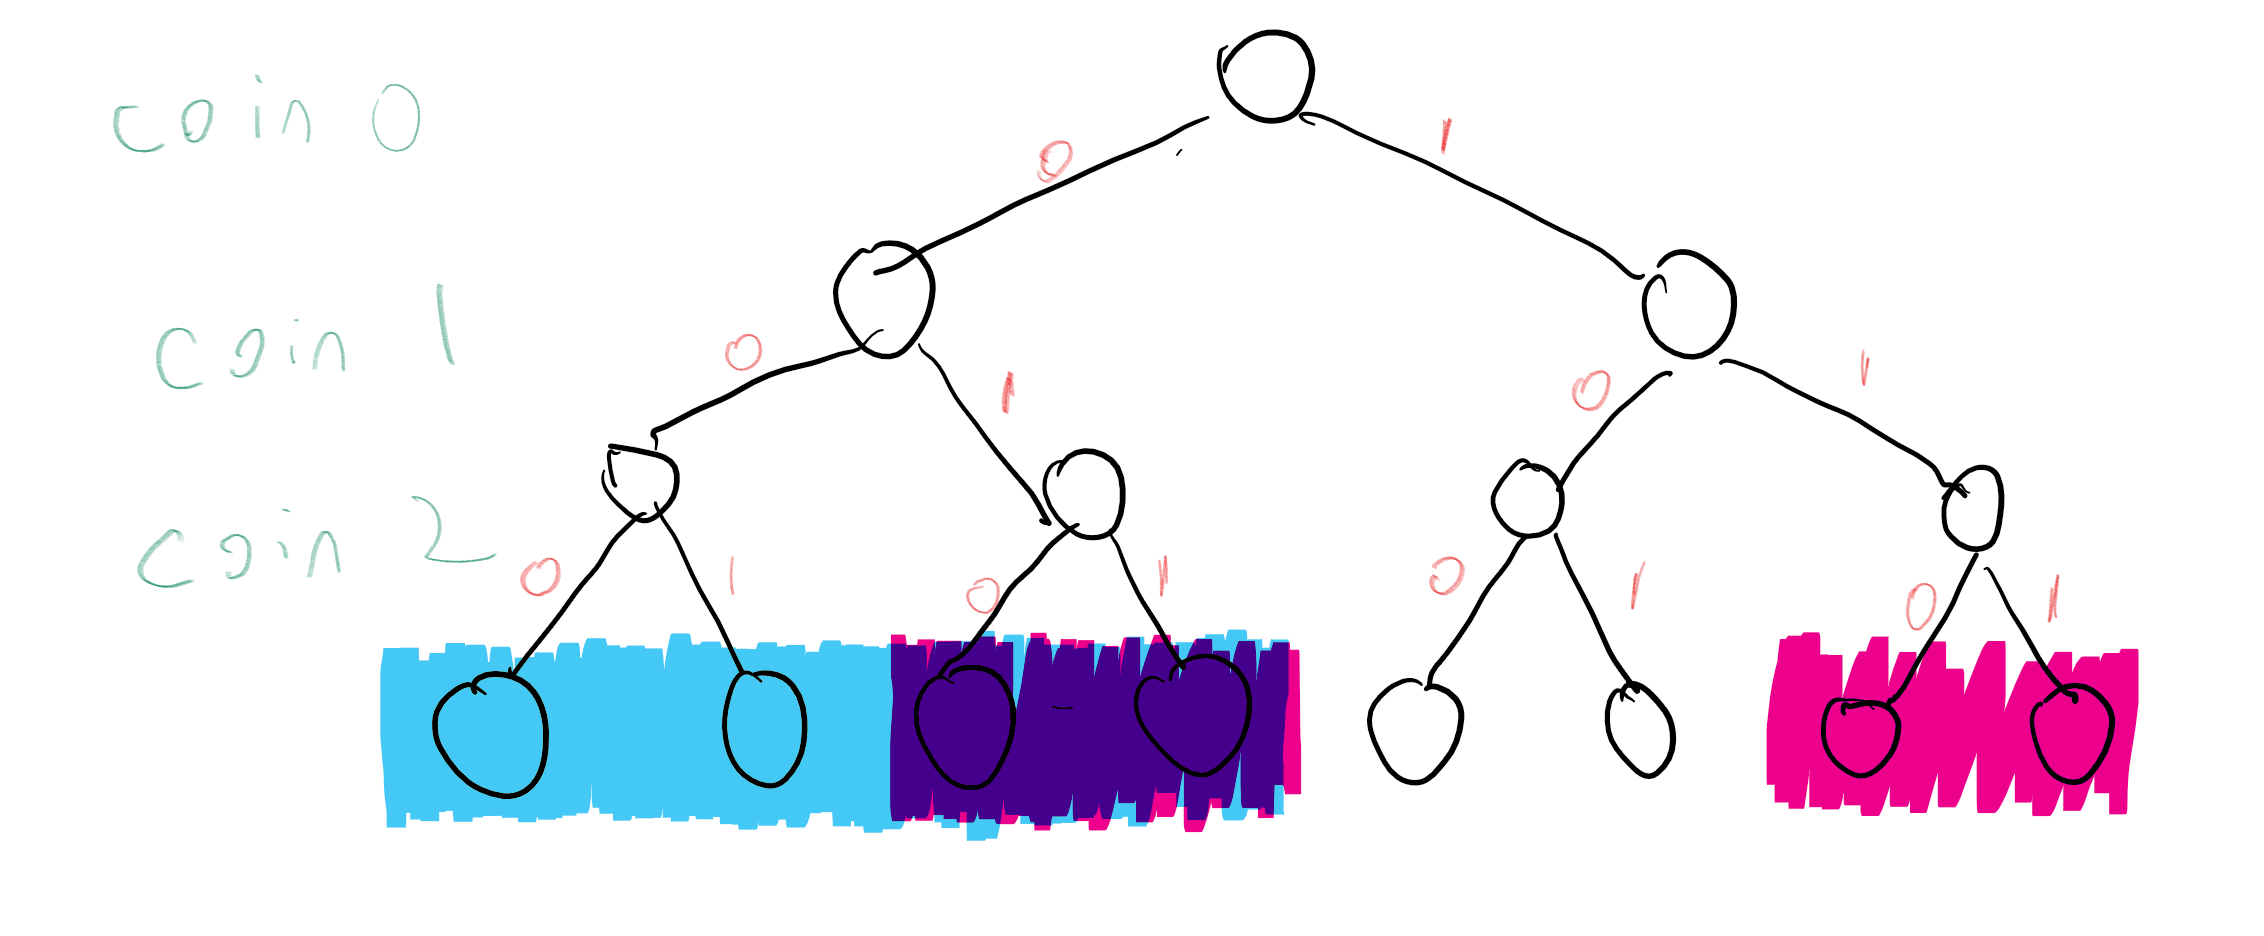
\includegraphics[width=\linewidth, height=1.5in, keepaspectratio]{../figure/coinexperiment.png}
\caption{The probabilistic experiment of tossing three coins corresponds
to making \(2\times 2 \times 2 = 8\) choices, each with equal
probability. In this example, the blue set corresponds to the event
\(A = \{ x\in \{0,1\}^3 \;|\; x_0 = 0 \}\) where the first coin toss is
equal to \(0\), and the pink set corresponds to the event
\(B = \{ x\in \{0,1\}^3 \;|\; x_1 = 1 \}\) where the second coin toss is
equal to \(1\) (with their intersection having a purplish color). As we
can see, each of these events contains \(4\) elements (out of \(8\)
total) and so has probability \(1/2\). The intersection of \(A\) and
\(B\) contains two elements, and so the probability that both of these
events occur is \(2/8 = 1/4\).}
\label{coinexperimentfig}
\end{marginfigure}

An \emph{event} is simply a subset \(A\) of \(\{0,1\}^n\). The
\emph{probability of \(A\)}, denoted by \(\Pr_{x\sim \{0,1\}^n}[A]\) (or
\(\Pr[A]\) for short, when the sample space is understood from the
context), is the probability that an \(x\) chosen uniformly at random
will be contained in \(A\). Note that this is the same as \(|A|/2^n\)
(where \(|A|\) as usual denotes the number of elements in the set
\(A\)). For example, the probability that \(x\) has an even number of
ones is \(\Pr[A]\) where
\(A=\{ x : \sum_{i=0}^{n-1} x_i \;= 0 \mod 2 \}\). In the case \(n=3\),
\(A=\{ 000,011,101,110 \}\), and hence
\(\Pr[A]=\tfrac{4}{8}=\tfrac{1}{2}\) (see \cref{eventhreecoinsfig}). It
turns out this is true for every \(n\):

\begin{marginfigure}
\centering
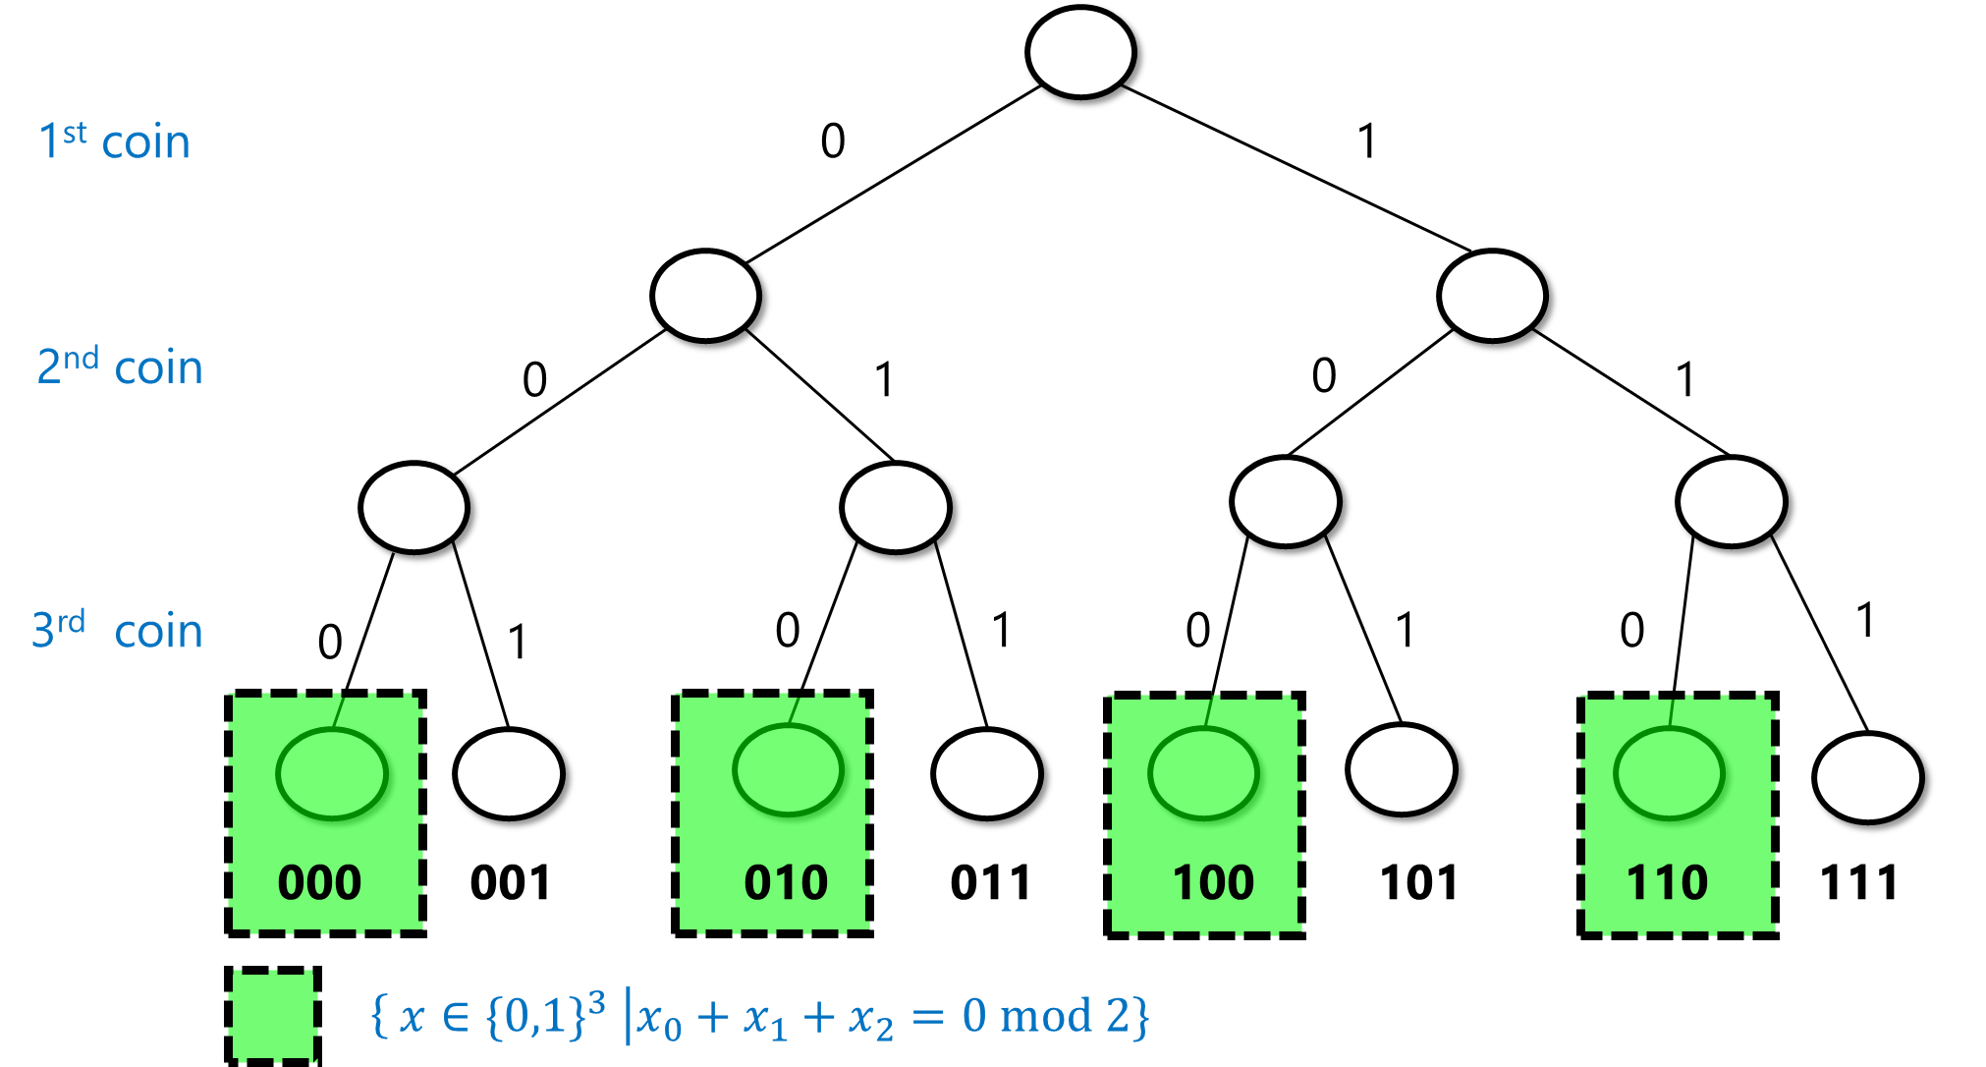
\includegraphics[width=\linewidth, height=1.5in, keepaspectratio]{../figure/even3coins.png}
\caption{The event that if we toss three coins
\(x_0,x_1,x_2 \in \{0,1\}\) then the sum of the \(x_i\)'s is even has
probability \(1/2\) since it corresponds to exactly \(4\) out of the
\(8\) possible strings of length \(3\).}
\label{eventhreecoinsfig}
\end{marginfigure}

\hypertarget{evenprob}{}
\begin{lemma} \label[lemma]{evenprob}

For every \(n>0\),
\begin{equation*}
\Pr_{x\sim \{0,1\}^n}[ \text{$\sum_{i=0}^{n-1} x_i$ is even }] = 1/2
\end{equation*}

\end{lemma}

\begin{pause} \label[pause]{0-To-test-your-intuition}

To test your intuition on probability, try to stop here and prove the
lemma on your own.

\end{pause}

\begin{proof}[Proof of \cref{evenprob}] \label[proof]{0-We-prove-the-lemma-by-}

We prove the lemma by induction on \(n\). For the case \(n=1\) it is
clear since \(x=0\) is even and \(x=1\) is odd, and hence the
probability that \(x\in \{0,1\}\) is even is \(1/2\). Let \(n>1\). We
assume by induction that the lemma is true for \(n-1\) and we will prove
it for \(n\). We split the set \(\{0,1\}^n\) into four disjoint sets
\(E_0,E_1,O_0,O_1\), where for \(b\in \{0,1\}\), \(E_b\) is defined as
the set of \(x\in \{0,1\}^n\) such that \(x_0\cdots x_{n-2}\) has even
number of ones and \(x_{n-1}=b\) and similarly \(O_b\) is the set of
\(x\in \{0,1\}^n\) such that \(x_0 \cdots x_{n-2}\) has odd number of
ones and \(x_{n-1}=b\). Since \(E_0\) is obtained by simply extending
\(n-1\)-length string with even number of ones by the digit \(0\), the
size of \(E_0\) is simply the number of such \(n-1\)-length strings
which by the induction hypothesis is \(2^{n-1}/2 = 2^{n-2}\). The same
reasoning applies for \(E_1\), \(O_0\), and \(O_1\). Hence each one of
the four sets \(E_0,E_1,O_0,O_1\) is of size \(2^{n-2}\). Since
\(x\in \{0,1\}^n\) has an even number of ones if and only if
\(x \in E_0 \cup O_1\) (i.e., either the first \(n-1\) coordinates sum
up to an even number and the final coordinate is \(0\) or the first
\(n-1\) coordinates sum up to an odd number and the final coordinate is
\(1\)), we get that the probability that \(x\) satisfies this property
is
\begin{equation*}

\tfrac{|E_0\cup O_1|}{2^n} = \frac{2^{n-2}+2^{n-2}}{2^n} = \frac{1}{2} \;,

\end{equation*}
using the fact that \(E_0\) and \(O_1\) are disjoint and hence
\(|E_0 \cup O_1| = |E_0|+|O_1|\).

\end{proof}

We can also use the \emph{intersection} (\(\cap\)) and \emph{union}
(\(\cup\)) operators to talk about the probability of both event \(A\)
\emph{and} event \(B\) happening, or the probability of event \(A\)
\emph{or} event \(B\) happening. For example, the probability \(p\) that
\(x\) has an \emph{even} number of ones \emph{and} \(x_0=1\) is the same
as \(\Pr[A\cap B]\) where
\(A=\{ x\in \{0,1\}^n : \sum_{i=0}^{n-1} x_i =0 \mod 2 \}\) and
\(B=\{ x\in \{0,1\}^n : x_0 = 1 \}\). This probability is equal to
\(1/4\) for \(n > 1\). (It is a great exercise for you to pause here and
verify that you understand why this is the case.)

Because intersection corresponds to considering the logical AND of the
conditions that two events happen, while union corresponds to
considering the logical OR, we will sometimes use the \(\wedge\) and
\(\vee\) operators instead of \(\cap\) and \(\cup\), and so write this
probability \(p=\Pr[A \cap B]\) defined above also as
\begin{equation*}

\Pr_{x\sim \{0,1\}^n} \left[ \sum_i x_i =0 \mod 2 \; \wedge \; x_0 = 1 \right] \;.

\end{equation*}

If \(A \subseteq \{0,1\}^n\) is an event, then
\(\overline{A} = \{0,1\}^n \setminus A\) corresponds to the event that
\(A\) does \emph{not} happen. Since \(|\overline{A}|=2^n-|A|\), we get
that
\begin{equation*}
\Pr[\overline{A}] = \tfrac{|\overline{A}|}{2^n} = \tfrac{2^n-|A|}{2^n}=1-\tfrac{|A|}{2^n} = 1- \Pr[A]

\end{equation*}
This makes sense: since \(A\) happens if and only if \(\overline{A}\)
does \emph{not} happen, the probability of \(\overline{A}\) should be
one minus the probability of \(A\).

\hypertarget{samplespace}{}
\begin{remark}[Remember the sample space] \label[remark]{samplespace}

While the above definition might seem very simple and almost trivial,
the human mind seems not to have evolved for probabilistic reasoning,
and it is surprising how often people can get even the simplest settings
of probability wrong. One way to make sure you don't get confused when
trying to calculate probability statements is to always ask yourself the
following two questions: \textbf{(1)} Do I understand what is the
\textbf{sample space} that this probability is taken over?, and
\textbf{(2)} Do I understand what is the definition of the
\textbf{event} that we are analyzing?.

For example, suppose that I were to randomize seating in my course, and
then it turned out that students sitting in row 7 performed better on
the final: how surprising should we find this? If we started out with
the hypothesis that there is something special about the number 7 and
chose it ahead of time, then the event that we are discussing is the
event \(A\) that students sitting in number 7 had better performance on
the final, and we might find it surprising. However, if we first looked
at the results and then chose the row whose average performance is best,
then the event we are discussing is the event \(B\) that there exists
\emph{some} row where the performance is higher than the overall
average. \(B\) is a superset of \(A\), and its probability (even if
there is no correlation between sitting and performance) can be quite
significant.

\end{remark}

\subsection{Random variables}\label{0-Random-variables}

\emph{Events} correspond to Yes/No questions, but often we want to
analyze finer questions. For example, if we make a bet at the roulette
wheel, we don't want to just analyze whether we won or lost, but also
\emph{how much} we've gained. A (real valued) \emph{random variable} is
simply a way to associate a number with the result of a probabilistic
experiment. Formally, a random variable is a function
\(X:\{0,1\}^n \rightarrow \R\) that maps every outcome
\(x\in \{0,1\}^n\) to an element \(X(x) \in \R\). For example, the
function \(sum:\{0,1\}^n \rightarrow \R\) that maps \(x\) to the sum of
its coordinates (i.e., to \(\sum_{i=0}^{n-1} x_i\)) is a random
variable.

The \emph{expectation} of a random variable \(X\), denoted by \(\E[X]\),
is the average value that that this number takes, taken over all draws
from the probabilistic experiment. In other words, the expectation of
\(X\) is defined as follows:
\begin{equation*}

\E[X] = \sum_{x\in \{0,1\}^n} 2^{-n}X(x) \;.

\end{equation*}

If \(X\) and \(Y\) are random variables, then we can define \(X+Y\) as
simply the random variable that maps a point \(x\in \{0,1\}^n\) to
\(X(x)+Y(x)\). One basic and very useful property of the expectation is
that it is \emph{linear}:

\hypertarget{linearityexp}{}
\begin{lemma}[Linearity of expectation] \label[lemma]{linearityexp}

\begin{equation*}
 \E[ X+Y ] = \E[X] + \E[Y] 
\end{equation*}

\end{lemma}

\begin{proof} \label[proof]{0-beginequationbegingath}

\begin{equation*}

\begin{gathered}
\E [X+Y] = \sum_{x\in \{0,1\}^n}2^{-n}\left(X(x)+Y(x)\right) =  \\
\sum_{x\in \{0,1\}^b} 2^{-n}X(x) + \sum_{x\in \{0,1\}^b} 2^{-n}Y(x) = \\
\E[X] + \E[Y]
\end{gathered}

\end{equation*}

\end{proof}

Similarly, \(\E[kX] = k\E[X]\) for every \(k \in \R\). For example,
using the linearity of expectation, it is very easy to show that the
expectation of the sum of the \(x_i\)'s for \(x \sim \{0,1\}^n\) is
equal to \(n/2\). Indeed, if we write \(X= \sum_{i=0}^{n-1} x_i\) then
\(X= X_0 + \cdots + X_{n-1}\) where \(X_i\) is the random variable
\(x_i\). Since for every \(i\), \(\Pr[X_i=0] = 1/2\) and
\(\Pr[X_i=1]=1/2\), we get that
\(\E[X_i] = (1/2)\cdot 0 + (1/2)\cdot 1 = 1/2\) and hence
\(\E[X] = \sum_{i=0}^{n-1}\E[X_i] = n\cdot(1/2) = n/2\).

\begin{pause} \label[pause]{0-If-you-have-not-seen-d}

If you have not seen discrete probability before, please go over this
argument again until you are sure you follow it; it is a prototypical
simple example of the type of reasoning we will employ again and again
in this course.

\end{pause}

If \(A\) is an event, then \(1_A\) is the random variable such that
\(1_A(x)\) equals \(1\) if \(x\in A\), and \(1_A(x)=0\) otherwise. Note
that \(\Pr[A] = \E[1_A]\) (can you see why?). Using this and the
linearity of expectation, we can show one of the most useful bounds in
probability theory:

\hypertarget{unionbound}{}
\begin{lemma}[Union bound] \label[lemma]{unionbound}

For every two events \(A,B\), \(\Pr[ A \cup B] \leq \Pr[A]+\Pr[B]\)

\end{lemma}

\begin{pause} \label[pause]{0-Before-looking-at-the-}

Before looking at the proof, try to see why the union bound makes
intuitive sense. We can also prove it directly from the definition of
probabilities and the cardinality of sets, together with the equation
\(|A \cup B| \leq |A|+|B|\). Can you see why the latter equation is
true? (See also \cref{unionboundfig}.)

\end{pause}

\begin{proof}[Proof of \cref{unionbound}] \label[proof]{0-For-every-x-the-variab}

For every \(x\), the variable \(1_{A\cup B}(x) \leq 1_A(x)+1_B(x)\).
Hence,
\(\Pr[A\cup B] = \E[ 1_{A \cup B} ] \leq \E[1_A+1_B] = \E[1_A]+\E[1_B] = \Pr[A]+\Pr[B]\).

\end{proof}

The way we often use this in theoretical computer science is to argue
that, for example, if there is a list of 100 bad events that can happen,
and each one of them happens with probability at most \(1/10000\), then
with probability at least \(1-100/10000 = 0.99\), no bad event happens.

\begin{marginfigure}
\centering
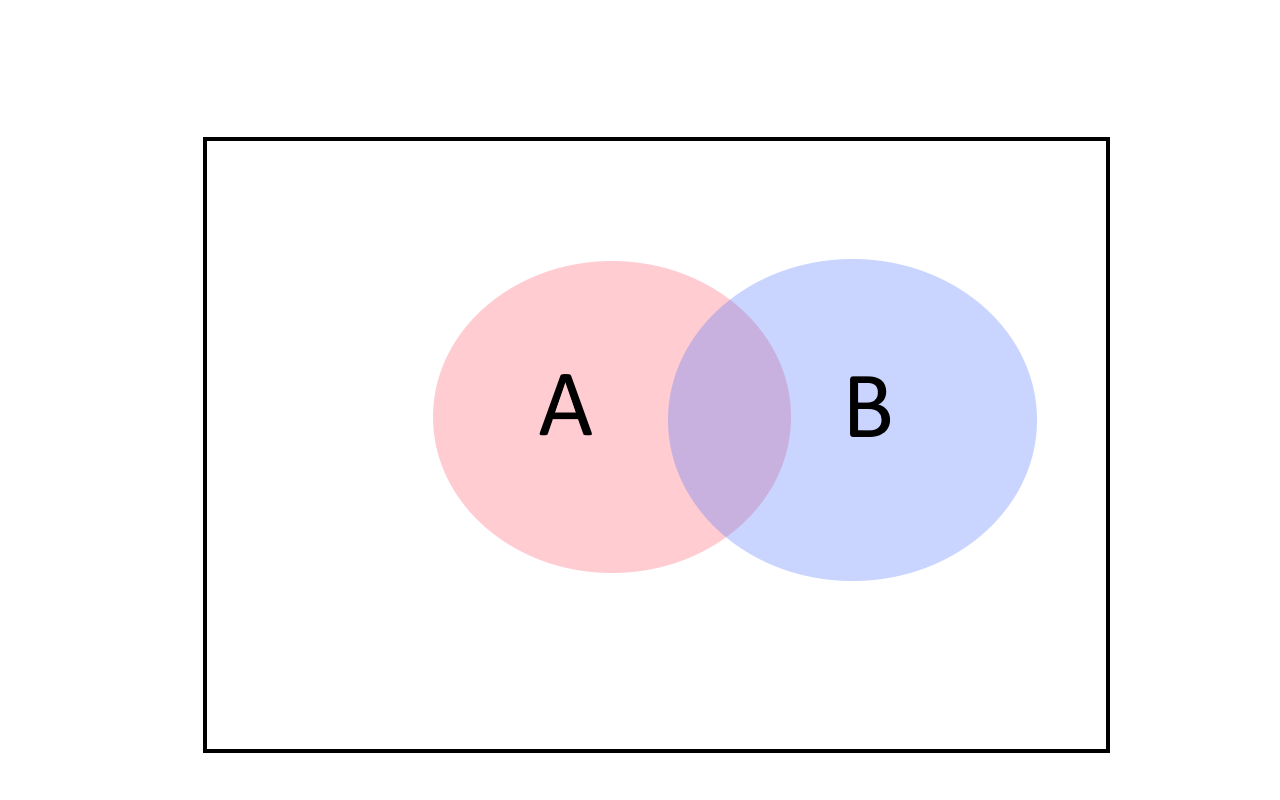
\includegraphics[width=\linewidth, height=1.5in, keepaspectratio]{../figure/unionbound.png}
\caption{The \emph{union bound} tells us that the probability of \(A\)
or \(B\) happening is at most the sum of the individual probabilities.
We can see it by noting that for every two sets
\(|A\cup B| \leq |A|+|B|\) (with equality only if \(A\) and \(B\) have
no intersection).}
\label{unionboundfig}
\end{marginfigure}

\subsection{Distributions over strings}\label{0-Distributions-over-str}

While most of the time we think of random variables as having as output
a \emph{real number}, we sometimes consider random variables whose
output is a \emph{string}. That is, we can think of a map
\(Y:\{0,1\}^n \rightarrow \{0,1\}^*\) and consider the ``random
variable'' \(Y\) such that for every \(y\in \{0,1\}^*\), the probability
that \(Y\) outputs \(y\) is equal to
\(\tfrac{1}{2^n}\left| \{ x \in \{0,1\}^n \;|\; Y(x)=y \}\right|\). To
avoid confusion, we will typically refer to such string-valued random
variables as \emph{distributions} over strings. So, a
\emph{distribution} \(Y\) over strings \(\{0,1\}^*\) can be thought of
as a finite collection of strings \(y_0,\ldots,y_{M-1} \in \{0,1\}^*\)
and probabilities \(p_0,\ldots,p_{M-1}\) (which are non-negative numbers
summing up to one), so that \(\Pr[ Y = y_i ] = p_i\).

Two distributions \(Y\) and \(Y'\) are \emph{identical} if they assign
the same probability to every string. For example, consider the
following two functions \(Y,Y':\{0,1\}^2 \rightarrow \{0,1\}^2\). For
every \(x \in \{0,1\}^2\), we define \(Y(x)=x\) and
\(Y'(x)=x_0(x_0\oplus x_1)\) where \(\oplus\) is the XOR operations.
Although these are two different functions, they induce the same
distribution over \(\{0,1\}^2\) when invoked on a uniform input. The
distribution \(Y(x)\) for \(x\sim \{0,1\}^2\) is of course the uniform
distribution over \(\{0,1\}^2\). On the other hand \(Y'\) is simply the
map \(00 \mapsto 00\), \(01 \mapsto 01\), \(10 \mapsto 11\),
\(11 \mapsto 10\) which is a permutation over the map
\(F:\{0,1\}^2 \rightarrow \{0,1\}^2\) defined as \(F(x_0x_1)=x_0x_1\)
and the map \(G:\{0,1\}^2 \rightarrow \{0,1\}^2\) defined as
\(G(x_0x_1)=x_0(x_0 \oplus x_1)\)

\subsection{More general sample spaces.}\label{0-More-general-sample-sp}

While in this chapter we assume that the underlying probabilistic
experiment corresponds to tossing \(n\) independent coins, everything we
say easily generalizes to sampling \(x\) from a more general finite or
countable set \(S\) (and not-so-easily generalizes to uncountable sets
\(S\) as well). A \emph{probability distribution} over a finite set
\(S\) is simply a function \(\mu : S \rightarrow [0,1]\) such that
\(\sum_{x\in S}\mu(s)=1\). We think of this as the experiment where we
obtain every \(x\in S\) with probability \(\mu(s)\), and sometimes
denote this as \(x\sim \mu\). An \emph{event} \(A\) is a subset of
\(S\), and the probability of \(A\), which we denote by \(\Pr_\mu[A]\),
is \(\sum_{x\in A} \mu(x)\). A \emph{random variable} is a function
\(X:S \rightarrow \R\), where the probability that \(X=y\) is equal to
\(\sum_{x\in S \text{ s.t. } X(x)=y} \mu(x)\).

\section{Correlations and independence}\label{0-Correlations-and-indep}

One of the most delicate but important concepts in probability is the
notion of \emph{independence} (and the opposing notion of
\emph{correlations}). Subtle correlations are often behind surprises and
errors in probability and statistical analysis, and several mistaken
predictions have been blamed on miscalculating the correlations between,
say, housing prices in Florida and Arizona, or voter preferences in Ohio
and Michigan. See also Joe Blitzstein's aptly named talk
\href{https://youtu.be/dzFf3r1yph8}{``Conditioning is the Soul of
Statistics''}. (Another thorny issue is of course the difference between
\emph{correlation} and \emph{causation}. Luckily, this is another point
we don't need to worry about in our clean setting of tossing \(n\)
coins.)

Two events \(A\) and \(B\) are \emph{independent} if the fact that \(A\)
happens makes \(B\) neither more nor less likely to happen. For example,
if we think of the experiment of tossing \(3\) random coins
\(x\in \{0,1\}^3\), and we let \(A\) be the event that \(x_0=1\) and
\(B\) the event that \(x_0 + x_1 + x_2 \geq 2\), then if \(A\) happens
it is more likely that \(B\) happens, and hence these events are
\emph{not} independent. On the other hand, if we let \(C\) be the event
that \(x_1=1\), then because the second coin toss is not affected by the
result of the first one, the events \(A\) and \(C\) are independent.

The formal definition is that events \(A\) and \(B\) are
\emph{independent} if \(\Pr[A \cap B]=\Pr[A] \cdot \Pr[B]\). If
\(\Pr[A \cap B] > \Pr[A]\cdot \Pr[B]\) then we say that \(A\) and \(B\)
are \emph{positively correlated}, while if
\(\Pr[ A \cap B] < \Pr[A] \cdot \Pr[B]\) then we say that \(A\) and
\(B\) are \emph{negatively correlated} (see \cref{coinexperimentfig}).

\begin{marginfigure}
\centering
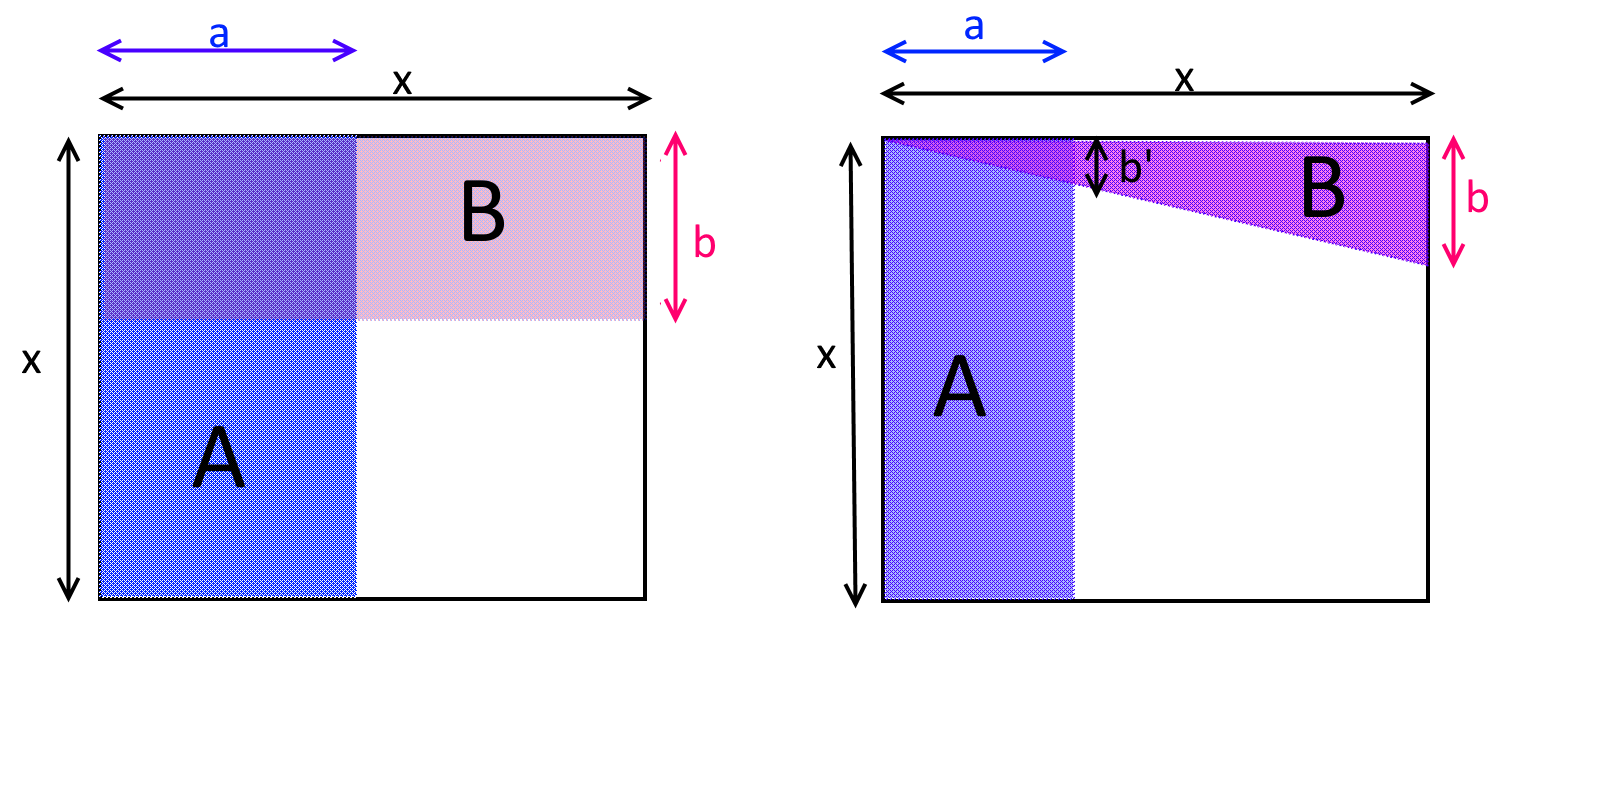
\includegraphics[width=\linewidth, height=1.5in, keepaspectratio]{../figure/independence.png}
\caption{Two events \(A\) and \(B\) are \emph{independent} if
\(\Pr[A \cap B]=\Pr[A]\cdot \Pr[B]\). In the two figures above, the
empty \(x\times x\) square is the sample space, and \(A\) and \(B\) are
two events in this sample space. In the left figure, \(A\) and \(B\) are
independent, while in the right figure they are negatively correlated,
since \(B\) is less likely to occur if we condition on \(A\) (and vice
versa). Mathematically, one can see this by noticing that in the left
figure the areas of \(A\) and \(B\) respectively are \(a\cdot x\) and
\(b\cdot x\), and so their probabilities are
\(\tfrac{a\cdot x}{x^2}=\tfrac{a}{x}\) and
\(\tfrac{b\cdot x}{x^2}=\tfrac{b}{x}\) respectively, while the area of
\(A \cap B\) is \(a\cdot b\) which corresponds to the probability
\(\tfrac{a\cdot b}{x^2}\). In the right figure, the area of the triangle
\(B\) is \(\tfrac{b\cdot x}{2}\) which corresponds to a probability of
\(\tfrac{b}{2x}\), but the area of \(A \cap B\) is
\(\tfrac{b' \cdot a}{2}\) for some \(b'<b\). This means that the
probability of \(A \cap B\) is
\(\tfrac{b'\cdot a}{2x^2} < \tfrac{b}{2x} \cdot \tfrac{a}{x}\), or in
other words \(\Pr[A \cap B ] < \Pr[A] \cdot \Pr[B]\).}
\label{independencefig}
\end{marginfigure}

If we consider the above examples on the experiment of choosing
\(x\in \{0,1\}^3\) then we can see that

\begin{equation*}

\begin{aligned}
\Pr[x_0=1] &= \tfrac{1}{2} \\
\Pr[x_0+x_1+x_2 \geq 2] = \Pr[\{ 011,101,110,111 \}] &= \tfrac{4}{8} = \tfrac{1}{2}
\end{aligned}

\end{equation*}

but

\begin{equation*}

\Pr[x_0 =1 \; \wedge \; x_0+x_1+x_2 \geq 2 ] = \Pr[ \{101,110,111 \} ] = \tfrac{3}{8} > \tfrac{1}{2} \cdot \tfrac{1}{2}

\end{equation*}

and hence, as we already observed, the events \(\{ x_0 = 1 \}\) and
\(\{ x_0+x_1+x_2 \geq 2 \}\) are not independent and in fact are
positively correlated. On the other hand,
\(\Pr[ x_0 = 1 \wedge x_1 = 1 ] = \Pr[ \{110,111 \}] = \tfrac{2}{8} = \tfrac{1}{2} \cdot \tfrac{1}{2}\)
and hence the events \(\{x_0 = 1 \}\) and \(\{ x_1 = 1 \}\) are indeed
independent.

\hypertarget{disjoint}{}
\begin{remark}[Disjointness vs independence] \label[remark]{disjoint}

People sometimes confuse the notion of \emph{disjointness} and
\emph{independence}, but these are actually quite different. Two events
\(A\) and \(B\) are \emph{disjoint} if \(A \cap B = \emptyset\), which
means that if \(A\) happens then \(B\) definitely does not happen. They
are \emph{independent} if \(\Pr[A \cap B]=\Pr[A]\Pr[B]\) which means
that knowing that \(A\) happens gives us no information about whether
\(B\) happened or not. If \(A\) and \(B\) have nonzero probability, then
being disjoint implies that they are \emph{not} independent, since in
particular it means that they are negatively correlated.

\end{remark}

\paragraph{Conditional probability:} If \(A\) and \(B\) are events, and
\(A\) happens with nonzero probability then we define the probability
that \(B\) happens \emph{conditioned on \(A\)} to be
\(\Pr[B|A] = \Pr[A \cap B]/\Pr[A]\). This corresponds to calculating the
probability that \(B\) happens if we already know that \(A\) happened.
Note that \(A\) and \(B\) are independent if and only if
\(\Pr[B|A]=\Pr[B]\).

\paragraph{More than two events:} We can generalize this definition to
more than two events. We say that events \(A_1,\ldots,A_k\) are
\emph{mutually independent} if knowing that any set of them occurred or
didn't occur does not change the probability that an event outside the
set occurs. Formally, the condition is that for every subset
\(I \subseteq [k]\),
\begin{equation*}

\Pr[ \wedge_{i\in I} A_i] =\prod_{i\in I} \Pr[A_i].

\end{equation*}

For example, if \(x\sim \{0,1\}^3\), then the events \(\{ x_0=1 \}\),
\(\{ x_1 = 1\}\) and \(\{x_2 = 1 \}\) are mutually independent. On the
other hand, the events \(\{x_0 = 1 \}\), \(\{x_1 = 1\}\) and
\(\{ x_0 + x_1 = 0 \mod 2 \}\) are \emph{not} mutually independent, even
though every pair of these events is independent (can you see why? see
also \cref{independencecoinsfig}).

\begin{marginfigure}
\centering
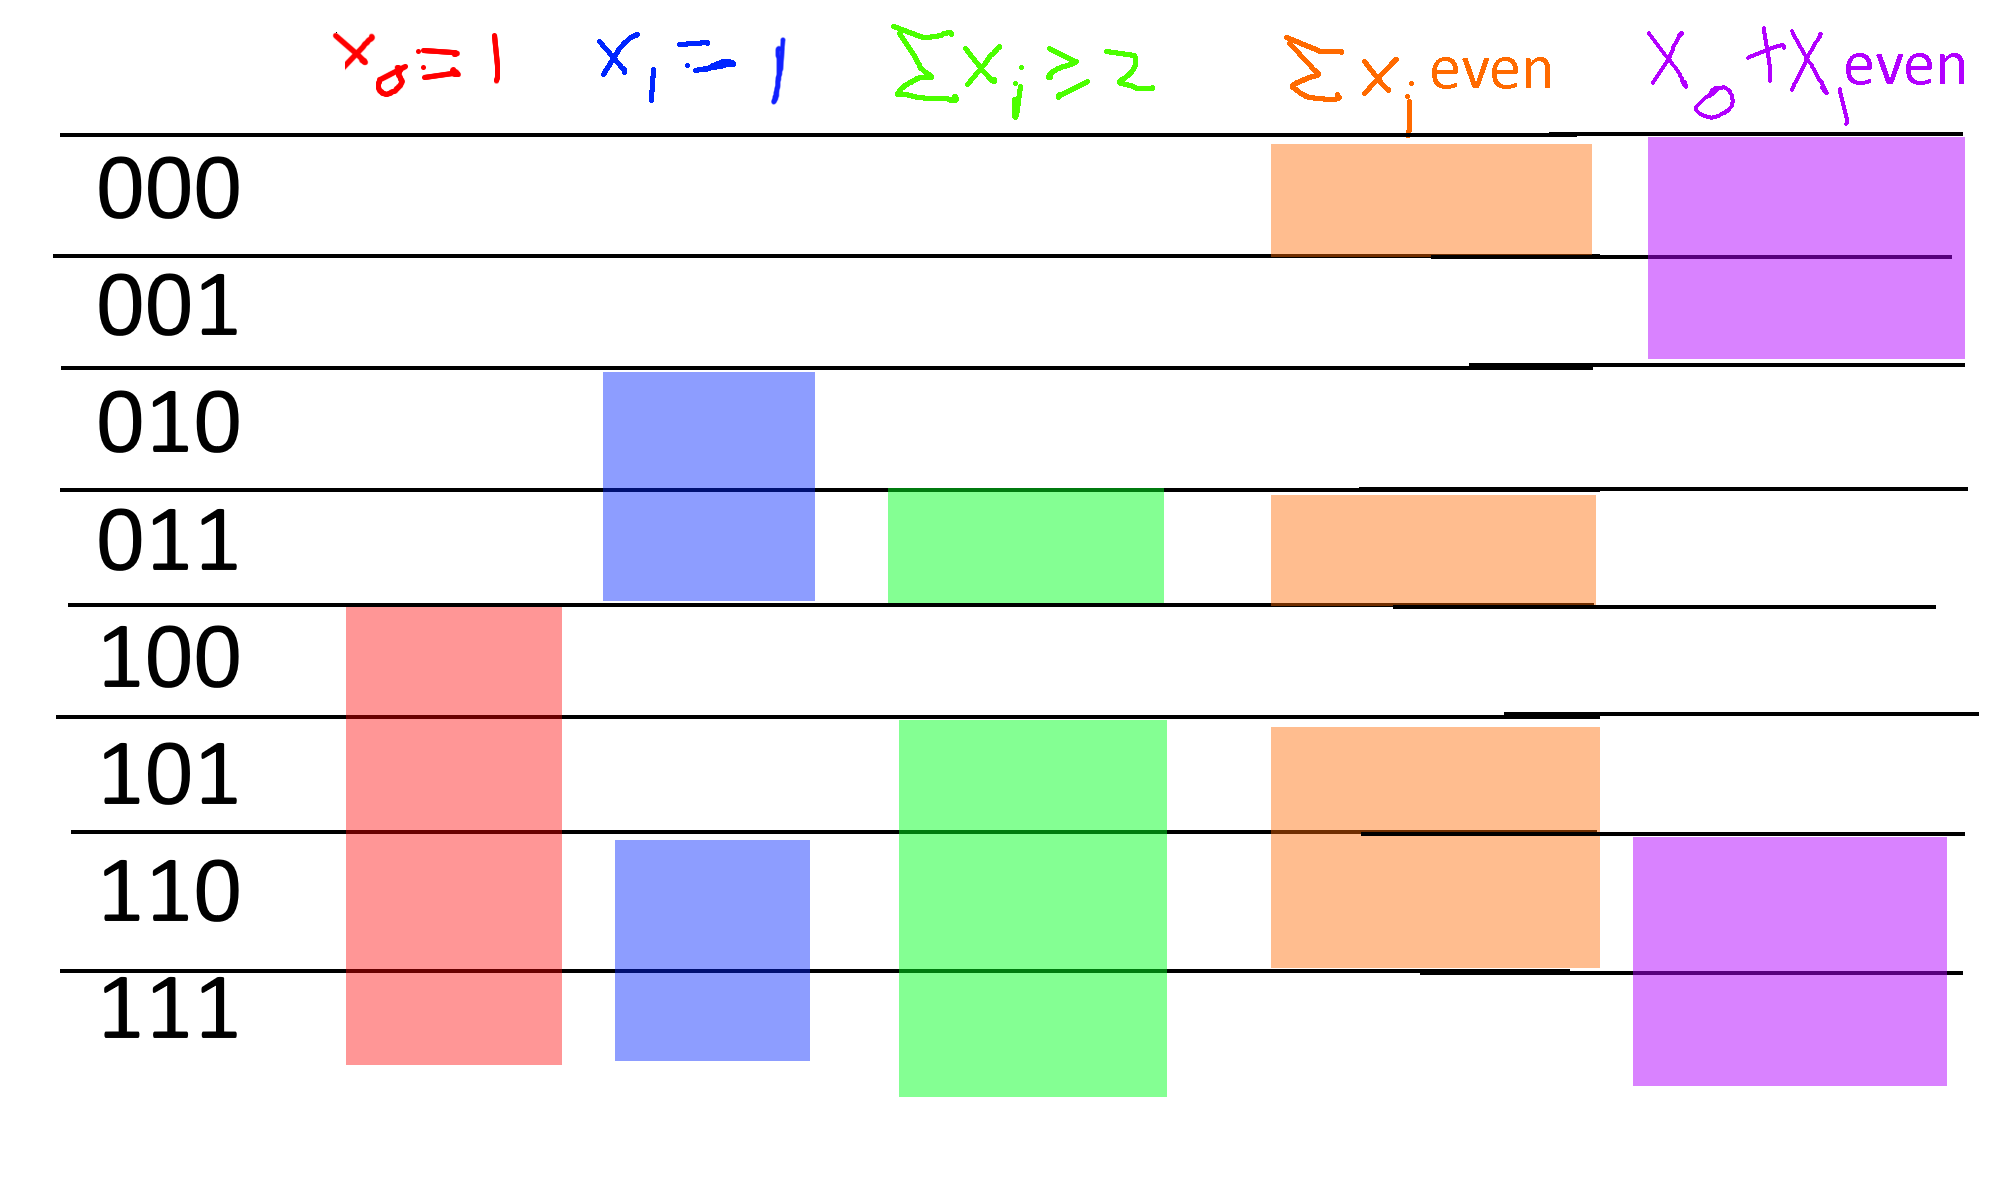
\includegraphics[width=\linewidth, height=1.5in, keepaspectratio]{../figure/independencecoins.png}
\caption{Consider the sample space \(\{0,1\}^n\) and the events
\(A,B,C,D,E\) corresponding to \(A\): \(x_0=1\), \(B\): \(x_1=1\),
\(C\): \(x_0+x_1+x_2 \geq 2\), \(D\): \(x_0+x_1+x_2 = 0 mod 2\) and
\(D\): \(x_0+x_1 = 0 mod 2\). We can see that \(A\) and \(B\) are
independent, \(C\) is positively correlated with \(A\) and positively
correlated with \(B\), the three events \(A,B,D\) are mutually
independent, and while every pair out of \(A,B,E\) is independent, the
three events \(A,B,E\) are not mutually independent since their
intersection has probability \(\tfrac{2}{8}=\tfrac{1}{4}\) instead of
\(\tfrac{1}{2}\cdot \tfrac{1}{2} \cdot \tfrac{1}{2} = \tfrac{1}{8}\).}
\label{independencecoinsfig}
\end{marginfigure}

\subsection{Independent random
variables}\label{0-Independent-random-var}

We say that two random variables \(X:\{0,1\}^n \rightarrow \R\) and
\(Y:\{0,1\}^n \rightarrow \R\) are independent if for every
\(u,v \in \R\), the events \(\{ X=u \}\) and \(\{ Y=v \}\) are
independent. (We use \(\{ X=u \}\) as shorthand for
\(\{ x \;|\; X(x)=u \}\).) In other words, \(X\) and \(Y\) are
independent if \(\Pr[ X=u \wedge Y=v]=\Pr[X=u]\Pr[Y=v]\) for every
\(u,v \in \R\). For example, if two random variables depend on the
result of tossing different coins then they are independent:

\hypertarget{indcoins}{}
\begin{lemma} \label[lemma]{indcoins}

Suppose that \(S=\{ s_0,\ldots, s_{k-1} \}\) and
\(T=\{ t_0 ,\ldots, t_{m-1} \}\) are disjoint subsets of
\(\{0,\ldots,n-1\}\) and let \(X,Y:\{0,1\}^n \rightarrow \R\) be random
variables such that \(X=F(x_{s_0},\ldots,x_{s_{k-1}})\) and
\(Y=G(x_{t_0},\ldots,x_{t_{m-1}})\) for some functions
\(F: \{0,1\}^k \rightarrow \R\) and \(G: \{0,1\}^m \rightarrow \R\).
Then \(X\) and \(Y\) are independent.

\end{lemma}

\begin{pause} \label[pause]{0-The-notation-in-the-le}

The notation in the lemma's statement is a bit cumbersome, but at the
end of the day, it simply says that if \(X\) and \(Y\) are random
variables that depend on two disjoint sets \(S\) and \(T\) of coins (for
example, \(X\) might be the sum of the first \(n/2\) coins, and \(Y\)
might be the largest consecutive stretch of zeroes in the second \(n/2\)
coins), then they are independent.

\end{pause}

\begin{proof}[Proof of \cref{indcoins}] \label[proof]{0-Let-abin-R-and-let-A--}

Let \(a,b\in \R\), and let \(A = \{ x \in \{0,1\}^k : F(x)=a \}\) and
\(B=\{ x\in \{0,1\}^m : F(x)=b \}\). Since \(S\) and \(T\) are disjoint,
we can reorder the indices so that \(S = \{0,\ldots,k-1\}\) and
\(T=\{k,\ldots,k+m-1\}\) without affecting any of the probabilities.
Hence we can write \(\Pr[X=a \wedge X=b] = |C|/2^n\) where
\(C= \{ x_0,\ldots,x_{n-1} : (x_0,\ldots,x_{k-1}) \in A \wedge (x_k,\ldots,x_{k+m-1}) \in B \}\).
Another way to write this using string concatenation is that
\(C = \{ xyz : x\in A, y\in B, z\in \{0,1\}^{n-k-m} \}\), and hence
\(|C|=|A||B|2^{n-k-m}\), which means that
\begin{equation*}

\tfrac{|C|}{2^n} = \tfrac{|A|}{2^k}\tfrac{|B|}{2^m}\tfrac{2^{n-k-m}}{2^{n-k-m}}=\Pr[X=a]\Pr[Y=b] .

\end{equation*}

\end{proof}

Note that if \(X\) and \(Y\) are independent random variables then (if
we let \(S_X,S_Y\) denote all the numbers that have positive probability
of being the output of \(X\) and \(Y\), respectively) it holds that:
\begin{equation*}

\begin{gathered}
\E[ \ensuremath{\mathit{XY}} ] = \sum_{a \in S_X,b \in S_Y} {\textstyle\Pr[X=a \wedge Y=b]}\cdot ab \; =^{(1)} \; \sum_{a \in S_X,b \in S_Y} {\textstyle \Pr[X=a]\Pr[Y=b]}\cdot ab =^{(2)} \\
\left(\sum_{a \in S_X} {\textstyle \Pr[X=a]}\cdot a\right)\left(\sum_{b \in S_Y} {\textstyle \Pr[Y=b]}b\right) =^{(3)} \\
\E[X] \E[Y]
\end{gathered}

\end{equation*}
where the first equality (\(=^{(1)}\)) follows from the independence of
\(X\) and \(Y\), the second equality (\(=^{(2)}\)) follows by ``opening
the parentheses'' of the righthand side, and the third inequality
(\(=^{(3)}\)) follows from the definition of expectation. (This is not
an ``if and only if''; see \cref{noindnocorex}.)

Another useful fact is that if \(X\) and \(Y\) are independent random
variables, then so are \(F(X)\) and \(G(Y)\) for all functions
\(F,G:\R \rightarrow R\). This is intuitively true since learning
\(F(X)\) can only provide us with less information than does learning
\(X\) itself. Hence, if learning \(X\) does not teach us anything about
\(Y\) (and so also about \(F(Y)\)) then neither will learning \(F(X)\).
Indeed, to prove this we can write for every \(a,b \in \R\):

\begin{equation*}

\begin{gathered}
\Pr[ F(X)=a \wedge G(Y)=b ] = \sum_{x \text{ s.t.} F(x)=a, y \text{ s.t. } G(y)=b} \Pr[ X=x \wedge Y=y ] = \\
\sum_{x \text{ s.t.} F(x)=a, y \text{ s.t. } G(y)=b} \Pr[ X=x ] \Pr[  Y=y ]  = \\
\left( \sum_{x \text{ s.t.} F(x)=a } \Pr[X=x ] \right) \cdot \left( \sum_{y \text{ s.t.} G(y)=b } \Pr[Y=y ] \right) = \\
\Pr[ F(X)=a] \Pr[G(Y)=b] .
\end{gathered}

\end{equation*}

\subsection{Collections of independent random
variables.}\label{0-Collections-of-indepen}

We can extend the notions of independence to more than two random
variables: we say that the random variables \(X_0,\ldots,X_{n-1}\) are
\emph{mutually independent} if for every \(a_0,\ldots,a_{n-1} \in \R\),
\begin{equation*}

\Pr\left[X_0=a_0 \wedge \cdots \wedge X_{n-1}=a_{n-1}\right]=\Pr[X_0=a_0]\cdots \Pr[X_{n-1}=a_{n-1}] .

\end{equation*}
And similarly, we have that

\hypertarget{expprod}{}
\begin{lemma}[Expectation of product of independent random variables] \label[lemma]{expprod}

If \(X_0,\ldots,X_{n-1}\) are mutually independent then
\begin{equation*}

\E[ \prod_{i=0}^{n-1} X_i ] = \prod_{i=0}^{n-1} \E[X_i] .

\end{equation*}

\end{lemma}

\hypertarget{indeplem}{}
\begin{lemma}[Functions preserve independence] \label[lemma]{indeplem}

If \(X_0,\ldots,X_{n-1}\) are mutually independent, and
\(Y_0,\ldots,Y_{n-1}\) are defined as \(Y_i = F_i(X_i)\) for some
functions \(F_0,\ldots,F_{n-1}:\R \rightarrow \R\), then
\(Y_0,\ldots,Y_{n-1}\) are mutually independent as well.

\end{lemma}

\begin{pause} \label[pause]{0-We-leave-proving-crefe}

We leave proving \cref{expprod} and \cref{indeplem} as \cref{expprodex}
\cref{indeplemex}. It is good idea for you stop now and do these
exercises to make sure you are comfortable with the notion of
independence, as we will use it heavily later on in this course.

\end{pause}

\section{Concentration and tail bounds}\label{0-Concentration-and-tail}

The name ``expectation'' is somewhat misleading. For example, suppose
that you and I place a bet on the outcome of 10 coin tosses, where if
they all come out to be \(1\)'s then I pay you 100,000 dollars and
otherwise you pay me 10 dollars. If we let
\(X:\{0,1\}^{10} \rightarrow \R\) be the random variable denoting your
gain, then we see that

\begin{equation*}

\E[X] = 2^{-10}\cdot 100000 - (1-2^{-10})10 \sim 90 .

\end{equation*}

But we don't really ``expect'' the result of this experiment to be for
you to gain 90 dollars. Rather, 99.9\% of the time you will pay me 10
dollars, and you will hit the jackpot 0.01\% of the times.

However, if we repeat this experiment again and again (with fresh and
hence \emph{independent} coins), then in the long run we do expect your
average earning to be close to 90 dollars, which is the reason why
casinos can make money in a predictable way even though every individual
bet is random. For example, if we toss \(n\) independent and unbiased
coins, then as \(n\) grows, the number of coins that come up ones will
be more and more \emph{concentrated} around \(n/2\) according to the
famous ``bell curve'' (see \cref{bellfig}).

\begin{marginfigure}
\centering
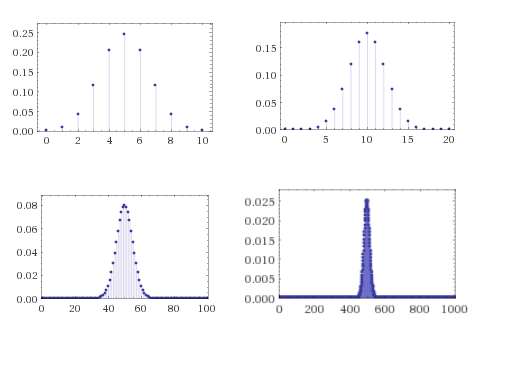
\includegraphics[width=\linewidth, height=1.5in, keepaspectratio]{../figure/binomial.png}
\caption{The probabilities that we obtain a particular sum when we toss
\(n=10,20,100,1000\) coins converge quickly to the Gaussian/normal
distribution.}
\label{bellfig}
\end{marginfigure}

Much of probability theory is concerned with so called
\emph{concentration} or \emph{tail} bounds, which are upper bounds on
the probability that a random variable \(X\) deviates too much from its
expectation. The first and simplest one of them is Markov's inequality:

\hypertarget{markovthm}{}
\begin{theorem}[Markov's inequality] \label[theorem]{markovthm}

If \(X\) is a non-negative random variable then
\(\Pr[ X \geq k \E[X] ] \leq 1/k\).

\end{theorem}

\begin{pause} \label[pause]{0-Markovs-Inequality-is-}

Markov's Inequality is actually a very natural statement (see also
\cref{markovfig}). For example, if you know that the average (not the
median!) household income in the US is 70,000 dollars, then in
particular you can deduce that at most 25 percent of households make
more than 280,000 dollars, since otherwise, even if the remaining 75
percent had zero income, the top 25 percent alone would cause the
average income to be larger than 70,000 dollars. From this example you
can already see that in many situations, Markov's inequality will not be
\emph{tight} and the probability of deviating from expectation will be
much smaller: see the Chebyshev and Chernoff inequalities below.

\end{pause}

\begin{proof}[Proof of \cref{markovthm}] \label[proof]{0-Let-mu--EX-and-define-}

Let \(\mu = \E[X]\) and define \(Y=1_{X \geq k \mu}\). That is,
\(Y(x)=1\) if \(X(x) \geq k \mu\) and \(Y(x)=0\) otherwise. Note that by
definition, for every \(x\), \(Y(x) \leq X/(k\mu)\). We need to show
\(\E[Y] \leq 1/k\). But this follows since
\(\E[Y] \leq \E[X/k(\mu)] = \E[X]/(k\mu) = \mu/(k\mu)=1/k\).

\end{proof}

\begin{marginfigure}
\centering
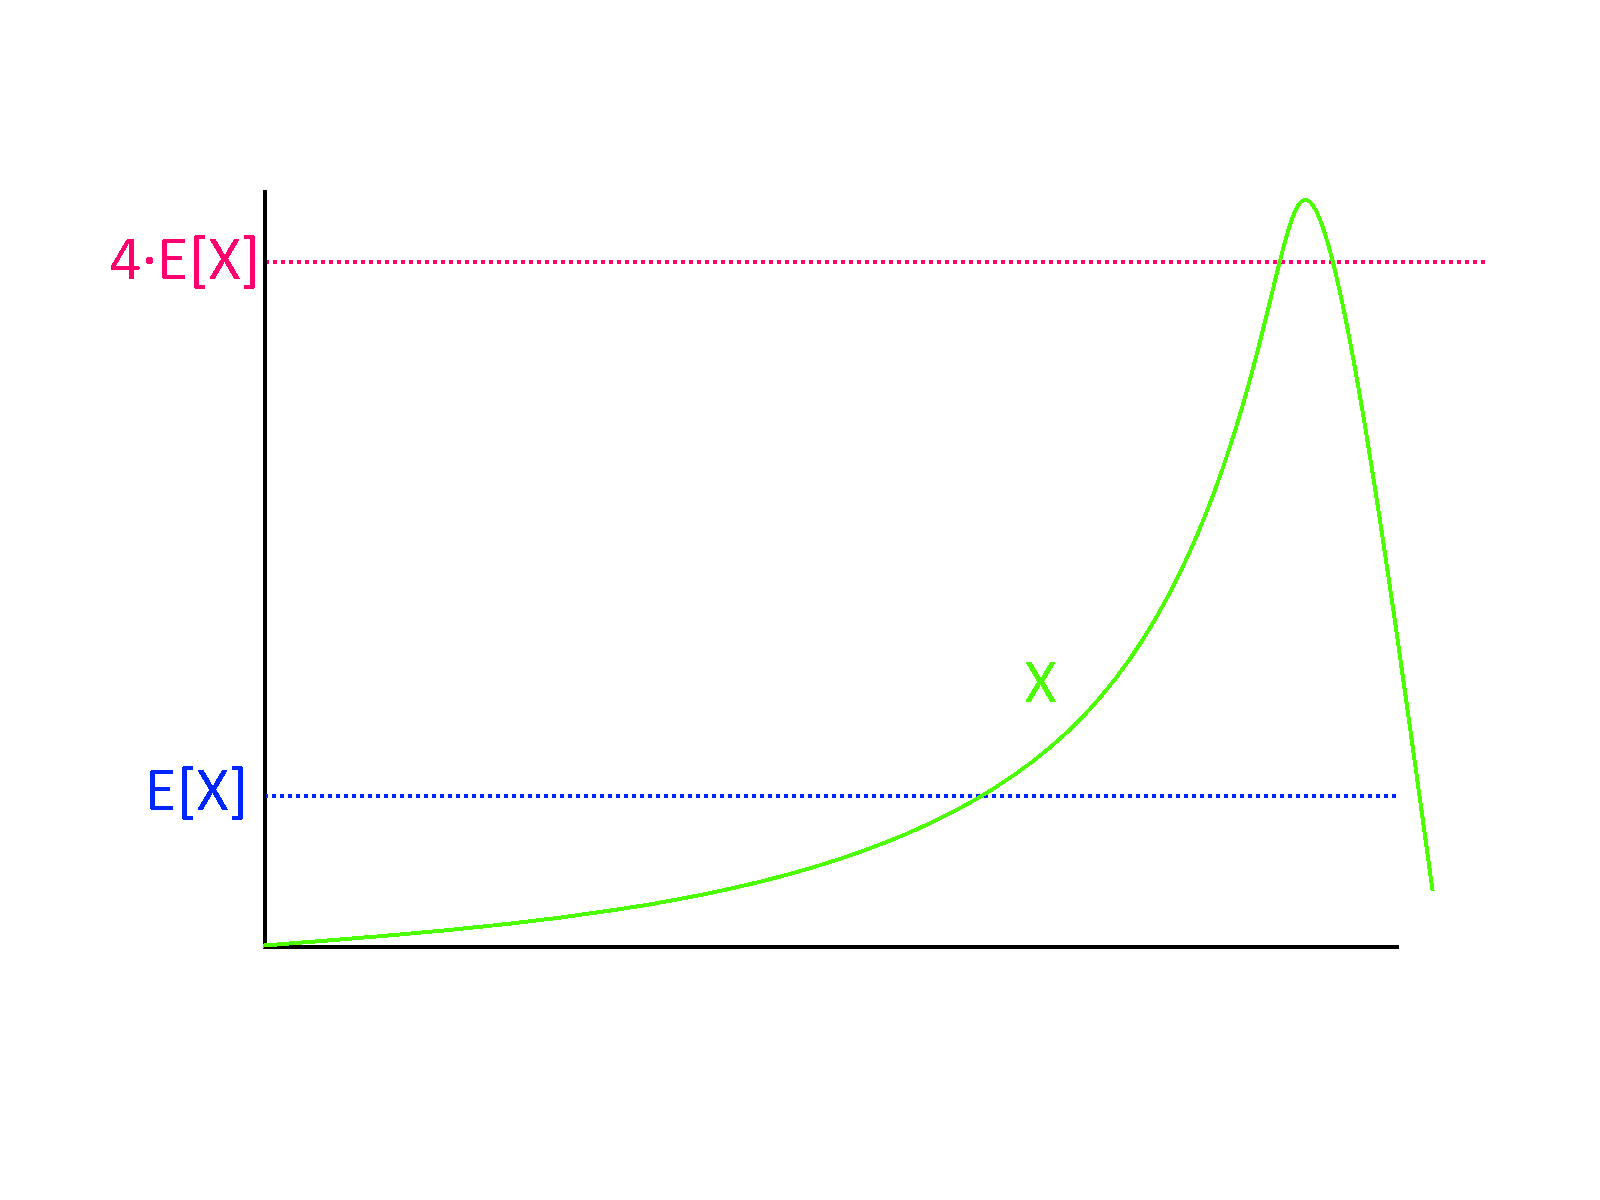
\includegraphics[width=\linewidth, height=1.5in, keepaspectratio]{../figure/markovineq.png}
\caption{Markov's Inequality tells us that a non-negative random
variable \(X\) cannot be much larger than its expectation, with high
probability. For example, if the expectation of \(X\) is \(\mu\), then
the probability that \(X>4\mu\) must be at most \(1/4\), as otherwise
just the contribution from this part of the sample space will be too
large.}
\label{markovfig}
\end{marginfigure}

\paragraph{Going beyond Markov’s Inequality:} Markov's inequality says
that a (non-negative) random variable \(X\) can't go too crazy and be,
say, a million times its expectation, with significant probability. But
ideally we would like to say that with high probability, \(X\) should be
very close to its expectation, e.g., in the range
\([0.99 \mu, 1.01 \mu]\) where \(\mu = \E[X]\). This is not generally
true, but does turn out to hold when \(X\) is obtained by combining
(e.g., adding) many independent random variables. This phenomenon,
variants of which are known as ``law of large numbers'', ``central limit
theorem'', ``invariance principles'' and ``Chernoff bounds'', is one of
the most fundamental in probability and statistics, and is one that we
heavily use in computer science as well.

\subsection{Chebyshev's Inequality}\label{0-Chebyshevs-Inequality}

A standard way to measure the deviation of a random variable from its
expectation is by using its \emph{standard deviation}. For a random
variable \(X\), we define the \emph{variance} of \(X\) as
\(\mathrm{Var}[X] = \E[(X-\mu)^2]\) where \(\mu = \E[X]\); i.e., the
variance is the average squared distance of \(X\) from its expectation.
The \emph{standard deviation} of \(X\) is defined as
\(\sigma[X] = \sqrt{\mathrm{Var}[X]}\). (This is well-defined since the
variance, being an average of a square, is always a non-negative
number.)

Using Chebyshev's inequality, we can control the probability that a
random variable is too many standard deviations away from its
expectation.

\hypertarget{chebychevthm}{}
\begin{theorem}[Chebyshev's inequality] \label[theorem]{chebychevthm}

Suppose that \(\mu=\E[X]\) and \(\sigma^2 = \mathrm{Var}[X]\). Then for
every \(k>0\), \(\Pr[ |X-\mu | \geq k \sigma ] \leq 1/k^2\).

\end{theorem}

\begin{proof} \label[proof]{0-The-proof-follows-from}

The proof follows from Markov's inequality. We define the random
variable \(Y = (X-\mu)^2\). Then \(\E[Y] = \mathrm{Var}[X] = \sigma^2\),
and hence by Markov the probability that \(Y > k^2\sigma^2\) is at most
\(1/k^2\). But clearly \((X-\mu)^2 \geq k^2\sigma^2\) if and only if
\(|X-\mu| \geq k\sigma\).

\end{proof}

One example of how to use Chebyshev's inequality is the setting when
\(X = X_1 + \cdots + X_n\) where \(X_i\)'s are \emph{independent and
identically distributed} (i.i.d for short) variables with values in
\([0,1]\) where each has expectation \(1/2\). Since
\(\E[X] = \sum_i \E[X_i] = n/2\), we would like to say that \(X\) is
very likely to be in, say, the interval \([0.499n,0.501n]\). Using
Markov's inequality directly will not help us, since it will only tell
us that \(X\) is very likely to be at most \(100n\) (which we already
knew, since it always lies between \(0\) and \(n\)). However, since
\(X_1,\ldots,X_n\) are independent, \[
\mathrm{Var}[X_1+\cdots +X_n] = \mathrm{Var}[X_1]+\cdots + \mathrm{Var}[X_n]  \label{varianceeq}\;.
\] (We leave showing this to the reader as \cref{varianceex}.)

For every random variable \(X_i\) in \([0,1]\),
\(\mathrm{Var}[X_i] \leq 1\) (if the variable is always in \([0,1]\), it
can't be more than \(1\) away from its expectation), and hence
\eqref{varianceeq} implies that \(\mathrm{Var}[X]\leq n\) and hence
\(\sigma[X] \leq \sqrt{n}\). For large \(n\), \(\sqrt{n} \ll 0.001n\),
and in particular if \(\sqrt{n} \leq 0.001n/k\), we can use Chebyshev's
inequality to bound the probability that \(X\) is not in
\([0.499n,0.501n]\) by \(1/k^2\).

\subsection{The Chernoff bound}\label{0-The-Chernoff-bound}

Chebyshev's inequality already shows a connection between independence
and concentration, but in many cases we can hope for a quantitatively
much stronger result. If, as in the example above, \(X= X_1+\ldots+X_n\)
where the \(X_i\)'s are bounded i.i.d random variables of mean \(1/2\),
then as \(n\) grows, the distribution of \(X\) would be roughly the
\emph{normal} or \emph{Gaussian} distribution\(-\) that is, distributed
according to the \emph{bell curve} (see \cref{bellfig} and
\cref{empiricalbellfig}). This distribution has the property of being
\emph{very} concentrated in the sense that the probability of deviating
\(k\) standard deviations from the mean is not merely \(1/k^2\) as is
guaranteed by Chebyshev, but rather is roughly \(e^{-k^2}\).
Specifically, for a normal random variable \(X\) of expectation \(\mu\)
and standard deviation \(\sigma\), the probability that
\(|X-\mu| \geq k\sigma\) is at most \(2e^{-k^2/2}\). That is, we have an
\emph{exponential decay} of the probability of deviation.

\begin{marginfigure}
\centering
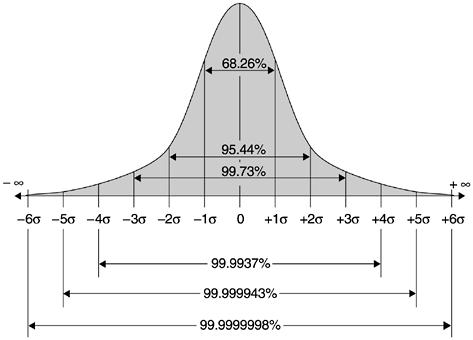
\includegraphics[width=\linewidth, height=1.5in, keepaspectratio]{../figure/sixsigma.jpg}
\caption{In the \emph{normal distribution} or the Bell curve, the
probability of deviating \(k\) standard deviations from the expectation
shrinks \emph{exponentially} in \(k^2\), and specifically with
probability at least \(1-2e^{-k^2/2}\), a random variable \(X\) of
expectation \(\mu\) and standard deviation \(\sigma\) satisfies
\(\mu -k\sigma \leq X \leq \mu+k\sigma\). This figure gives more precise
bounds for \(k=1,2,3,4,5,6\). (Image credit:Imran Baghirov)}
\label{empiricalbellfig}
\end{marginfigure}

The following extremely useful theorem shows that such exponential decay
occurs every time we have a sum of independent and bounded variables.
This theorem is known under many names in different communities, though
it is mostly called the
\href{https://en.wikipedia.org/wiki/Chernoff_bound}{Chernoff bound} in
the computer science literature:

\hypertarget{chernoffthm}{}
\begin{theorem}[Chernoff/Hoeffding bound] \label[theorem]{chernoffthm}

If \(X_1,\ldots,X_n\) are i.i.d random variables such that
\(X_i \in [0,1]\) and \(\E[X_i]=p\) for every \(i\), then for every
\(\epsilon >0\)
\begin{equation*}

\Pr[ \left| \sum_{i=0}^{n-1} X_i - pn \right| > \epsilon n ] \leq 2\cdot e^{-2\epsilon^2 n} .

\end{equation*}

\end{theorem}

We omit the proof, which appears in many texts, and uses Markov's
inequality on i.i.d random variables \(Y_0,\ldots,Y_n\) that are of the
form \(Y_i = e^{\lambda X_i}\) for some carefully chosen parameter
\(\lambda\). See \cref{chernoffstirlingex} for a proof of the simple
(but highly useful and representative) case where each \(X_i\) is
\(\{0,1\}\) valued and \(p=1/2\). (See also \cref{poorchernoff} for a
generalization.)

\section{Exercises}\label{0-Exercises}

\begin{exercise} \label[exercise]{0-Prove-that-for-every-f}

Prove that for every finite \(S,T\), there are \((|T|+1)^{|S|}\) partial
functions from \(S\) to \(T\).

\end{exercise}

\hypertarget{ohnotationex}{}
\begin{exercise}[$O$-notation] \label[exercise]{ohnotationex}

For every pair of functions \(F,G\) below, determine which of the
following relations holds: \(F=O(G)\), \(F=\Omega(G)\), \(F=o(G)\) or
\(F=\omega(G)\).

\begin{enumerate}
\def\labelenumi{\alph{enumi}.}
\item
  \(F(n)=n\), \(G(n)=100n\).
\item
  \(F(n)=n\), \(G(n)=\sqrt{n}\).
\item
  \(F(n)=n\log n\), \(G(n)=2^{(\log (n))^2}\).
\item
  \(F(n)=\sqrt{n}\), \(G(n)=2^{\sqrt{\log n}}\)
\item
  \(F(n) = \binom{n}{\ceil{0.2 n}}\) , \(G(n) = 2^{0.1 n}\) (where
  \(\binom{n}{k}\) is the number of \(k\)-sized subsets of a set of size
  \(n\)) and \(g(n) = 2^{0.1 n}\). See footnote for hint.\footnote{one
    way to do this is to use \href{https://goo.gl/cqEmS2}{Stirling's
    approximation for the factorial function.}.}
\end{enumerate}

\end{exercise}

\begin{exercise} \label[exercise]{0-Give-an-example-of-a-p}

Give an example of a pair of functions \(F,G:\N \rightarrow \N\) such
that neither \(F=O(G)\) nor \(G=O(F)\) holds.

\end{exercise}

\hypertarget{propexpecvariance}{}
\begin{exercise}[Properties of expectation and variance] \label[exercise]{propexpecvariance}

In the following exercise \(X,Y\) denote random variables over some
sample space \(S\). You can assume that the probability on \(S\) is the
uniform distribution--- every point \(s\) is output with probability
\(1/|S|\). Thus \({\mathbb{E}}[X]= (1/|S|)\sum_{s\in S}X(s)\). We define
the variance and standard deviation of \(X\) and \(Y\) as above (e.g.,
\(Var[X] = {\mathbb{E}}[(X-{\mathbb{E}}[X])^2 ]\) and the standard
deviation is the square root of the variance). You can reuse your
answers to prior questions in the later ones.

\begin{enumerate}
\def\labelenumi{\arabic{enumi}.}
\item
  Prove that \(Var[X]\) is always non-negative.
\item
  Prove that \(Var[X] = {\mathbb{E}}[X^2] - {\mathbb{E}}[X]^2\).
\item
  Prove that always \({\mathbb{E}}[X^2] \geq {\mathbb{E}}[X]^2\).
\item
  Give an example for a random variable \(X\) such that
  \({\mathbb{E}}[X^2] > {\mathbb{E}}[X]^2\).
\item
  Give an example for a random variable \(X\) such that its standard
  deviation is \emph{not equal} to
  \({\mathbb{E}}[ | X - {\mathbb{E}}[X] | ]\).
\item
  Give an example for a random variable \(X\) such that its standard
  deviation is \emph{equal to} to
  \({\mathbb{E}}[ | X - {\mathbb{E}}[X] | ]\).
\item
  Give an example for two random variables \(X,Y\) such that
  \({\mathbb{E}}[\ensuremath{\mathit{XY}}] = {\mathbb{E}}[X]{\mathbb{E}}[Y]\).
\item
  Give an example for two random variables \(X,Y\) such that
  \({\mathbb{E}}[\ensuremath{\mathit{XY}}] \neq {\mathbb{E}}[X]{\mathbb{E}}[Y]\).
\item
  Prove that if \(X\) and \(Y\) are independent random variables (i.e.,
  for every \(x,y\), \(\Pr[X=x \wedge Y=y]=\Pr[X=x]\Pr[Y=y]\)) then
  \({\mathbb{E}}[\ensuremath{\mathit{XY}}]={\mathbb{E}}[X]{\mathbb{E}}[Y]\)
  and \(Var[X+Y]=Var[X]+Var[Y]\).
\end{enumerate}

\end{exercise}

\hypertarget{randomfunction}{}
\begin{exercise}[Random hash function] \label[exercise]{randomfunction}

Suppose that \(H\) is chosen to be a random function mapping the numbers
\(\{1,\ldots,n\}\) to the numbers \(\{1,..,m \}\). That is, for every
\(i\in \{1,\ldots,n\}\), \(H(i)\) is chosen to be a random number in
\(\{ 1,\ldots, m\}\) and that choice is done independently for every
\(i\). For every \(i<j \in \{1,\ldots,n\}\), define the random variable
\(X_{i,j}\) to equal \(1\) if there was a \emph{collision} between
\(H(i)\) and \(H(j)\) in the sense that \(H(i)=H(j)\) and to equal \(0\)
otherwise.

\begin{enumerate}
\def\labelenumi{\arabic{enumi}.}
\item
  For every \(i<j\), compute \({\mathbb{E}}[ X_{i,j} ]\).
\item
  Define \(Y = \sum_{i<j} X_{i,j}\) to be the total number of
  collisions. Compute \({\mathbb{E}}[ Y ]\) as a function of \(n\) and
  \(m\). In particular your answer should imply that if \(m < n^2/1000\)
  then \({\mathbb{E}}[Y]>1\) and hence in expectation there should be at
  least one collision and so the function \(H\) will not be one to one.
\item
  Prove that if \(m > 1000\cdot n^2\) then the probability that \(H\) is
  one to one is at least \(0.9\).
\item
  Give an example of a random variable \(Z\) (unrelated to the function
  \(H\)) that is always equal to a non-negative integer, and such that
  \({\mathbb{E}}[Z] \geq 1000\) but \(\Pr[ Z > 0] < 0.001\).
\item
  Prove that if \(m < n^2/1000\) then the probability that \(H\) is one
  to one is at most \(0.1\).
\end{enumerate}

\end{exercise}

\section{Exercises}\label{0-Exercises}

\begin{exercise} \label[exercise]{0-Suppose-that-we-toss-t}

Suppose that we toss three independent fair coins \(a,b,c \in \{0,1\}\).
What is the probability that the XOR of \(a\),\(b\), and \(c\) is equal
to \(1\)? What is the probability that the AND of these three values is
equal to \(1\)? Are these two events independent?

\end{exercise}

\begin{exercise} \label[exercise]{0-Give-an-example-of-ran}

Give an example of random variables \(X,Y: \{0,1\}^3 \rightarrow \R\)
such that \(\E[\ensuremath{\mathit{XY}}] \neq \E[X]\E[Y]\).

\end{exercise}

\hypertarget{noindnocorex}{}
\begin{exercise} \label[exercise]{noindnocorex}

Give an example of random variables \(X,Y: \{0,1\}^3 \rightarrow \R\)
such that \(X\) and \(Y\) are \emph{not} independent but
\(\E[\ensuremath{\mathit{XY}}] =\E[X]\E[Y]\).

\end{exercise}

\hypertarget{expprodex}{}
\begin{exercise}[Product of expectations] \label[exercise]{expprodex}

Prove \cref{expprod}

\end{exercise}

\hypertarget{indeplemex}{}
\begin{exercise}[Transformations preserve independence] \label[exercise]{indeplemex}

Prove \cref{indeplem}

\end{exercise}

\hypertarget{varianceex}{}
\begin{exercise}[Variance of independent random variables] \label[exercise]{varianceex}

Prove that if \(X_0,\ldots,X_{n-1}\) are independent random variables
then
\(\mathrm{Var}[X_0+\cdots+X_{n-1}]=\sum_{i=0}^{n-1} \mathrm{Var}[X_i]\).

\end{exercise}

\hypertarget{entropyex}{}
\begin{exercise}[Entropy (challenge)] \label[exercise]{entropyex}

Recall the definition of a distribution \(\mu\) over some finite set
\(S\). Shannon defined the \emph{entropy} of a distribution \(\mu\),
denoted by \(H(\mu)\), to be \(\sum_{x\in S} \mu(x)\log(1/\mu(x))\). The
idea is that if \(\mu\) is a distribution of entropy \(k\), then
encoding members of \(\mu\) will require \(k\) bits, in an amortized
sense. In this exercise we justify this definition. Let \(\mu\) be such
that \(H(\mu)=k\).\\
1. Prove that for every one to one function
\(F:S \rightarrow \{0,1\}^*\), \(\E_{x \sim \mu} |F(x)| \geq k\).\\
2. Prove that for every \(\epsilon\), there is some \(n\) and a
one-to-one function \(F:S^n \rightarrow \{0,1\}^*\), such that
\(\E_{x\sim \mu^n} |F(x)| \leq n(k+\epsilon)\), where \(x \sim \mu\)
denotes the experiments of choosing \(x_0,\ldots,x_{n-1}\) each
independently from \(S\) using the distribution \(\mu\).

\end{exercise}

\hypertarget{entropybinomex}{}
\begin{exercise}[Entropy approximation to binomial] \label[exercise]{entropybinomex}

Let \(H(p) = p \log(1/p)+(1-p)\log(1/(1-p))\).\footnote{While you don't
  need this to solve this exercise, this is the function that maps \(p\)
  to the entropy (as defined in \cref{entropyex}) of the \(p\)-biased
  coin distribution over \(\{0,1\}\), which is the function
  \(\mu:\{0,1\}\rightarrow [0,1]\) s.y. \(\mu(0)=1-p\) and \(\mu(1)=p\).}

Prove that for every \(p \in (0,1)\) and \(\epsilon>0\), if \(n\) is
large enough then\footnote{\textbf{Hint:} Use Stirling's formula for
  approximating the factorial function.}
\begin{equation*}

2^{(H(p)-\epsilon)n }\binom{n}{pn} \leq 2^{(H(p)+\epsilon)n}

\end{equation*}
where \(\binom{n}{k}\) is the binomial coefficient
\(\tfrac{n!}{k!(n-k)!}\) which is equal to the number of \(k\)-size
subsets of \(\{0,\ldots,n-1\}\).

\end{exercise}

\hypertarget{chernoffstirlingex}{}
\begin{exercise}[Chernoff using Stirling] \label[exercise]{chernoffstirlingex}

\begin{enumerate}
\def\labelenumi{\arabic{enumi}.}
\item
  Prove that
  \(\Pr_{x\sim \{0,1\}^n}[ \sum x_i = k ] = \binom{n}{k}2^{-n}\).\\
\item
  Use this and \cref{entropybinomex} to prove (an approximate version
  of) the Chernoff bound for the case that \(X_0,\ldots,X_{n-1}\) are
  i.i.d. random variables over \(\{0,1\}\) each equaling \(0\) and \(1\)
  with probability \(1/2\). That is, prove that for every
  \(\epsilon>0\), and \(X_0,\ldots,X_{n-1}\) as above,
  \(\Pr[ |\sum_{i=0}^{n-1} - \tfrac{n/2}| > \epsilon n] < 2^{0.1 \cdot \epsilon^2 n}\).
\end{enumerate}

\end{exercise}

\hypertarget{poorchernoff}{}
\begin{exercise}[Poor man's Chernoff] \label[exercise]{poorchernoff}

\cref{chernoffstirlingex} establishes the Chernoff bound for the case
that \(X_0,\ldots,X_{n-1}\) are i.i.d variables over \(\{0,1\}\) with
expectation \(1/2\). In this exercise we use a slightly different method
(bounding the \emph{moments} of the random variables) to establish a
version of Chernoff where the random variables range over \([0,1]\) and
their expectation is some number \(p \in [0,1]\) that may be different
than \(1/2\). Let \(X_0,\ldots,X_{n-1}\) be i.i.d random variables with
\(\E X_i = p\) and \(\Pr [ 0 \leq X_i \leq 1 ]=1\). Define
\(Y_i = X_i - p\).

\begin{enumerate}
\def\labelenumi{\arabic{enumi}.}
\item
  Prove that for every \(j_0,\ldots,j_{n-1} \in \N\), if there exists
  one \(i\) such that \(j_i\) is odd then
  \(\E [\prod_{i=0}^{n-1} Y_i^{j_i}] = 0\).\\
\item
  Prove that for every \(k\),
  \(\E[ (\sum_{i=0}^{n-1} Y_i)^k ] \leq (10kn)^{k/2}\).\footnote{\textbf{Hint:}
    Bound the number of tuples \(j_0,\ldots,j_{n-1}\) such that every
    \(j_i\) is even and \(\sum j_i = k\) using the Binomial coefficient
    and the fact that in any such tuple there are at most \(k/2\)
    distinct indices.}\\
\item
  Prove that for every \(\epsilon>0\),
  \(\Pr[ |\sum_i Y_i| \geq \epsilon n ] \geq 2^{-\epsilon^2 n / (10000\log 1/\epsilon)}\).\footnote{\textbf{Hint:}
    Set \(k=2\lceil \epsilon^2 n /1000 \rceil\) and then show that if
    the event \(|\sum Y_i | \geq \epsilon n\) happens then the random
    variable \((\sum Y_i)^k\) is a factor of \(\epsilon^{-k}\) larger
    than its expectation.}
\end{enumerate}

\end{exercise}

\hypertarget{lowerboundcoins}{}
\begin{exercise}[Lower bound for distinguishing coins] \label[exercise]{lowerboundcoins}

The Chernoff bound can be used to show that if you were given a coin of
bias at least \(\epsilon\), you should only need \(O(1/\epsilon^2)\)
samples to be able to reject the ``null hypothesis'' that the coin is
completely unbiased with extremely high confidence. In the following
somewhat more challenging question, we try to show a converse to this,
proving that distinguishing between a fair every coin and a coin that
outputs ``heads'' with probability \(1/2 + \epsilon\) requires at least
\(\Omega(1/\epsilon^2)\) samples.

Let \(P\) be the uniform distribution over \({\{0,1\}}^n\) and \(Q\) be
the \(1/2+\epsilon\)-biased distribution corresponding to tossing \(n\)
coins in which each one has a probability of \(1/2+\epsilon\) of
equalling \(1\) and probability \(1/2-\epsilon\) of equalling \(0\).
Namely the probability of \(x\in{\{0,1\}}^n\) according to \(Q\) is
equal to \(\prod_{i=1}^n (1/2 - \epsilon + 2\epsilon x_i)\).

\begin{enumerate}
\def\labelenumi{\arabic{enumi}.}
\item
  Prove that for every threshold \(\theta\) between \(0\) and \(n\), if
  \(n < 1/(100\epsilon)^2\) then the probabilities that
  \(\sum x_i \leq \theta\) under \(P\) and \(Q\) respectively differ by
  at most \(0.1\). Therefore, one cannot use the test whether the number
  of heads is above or below some threshold to reliably distinguish
  between these two possibilities unless the number of samples \(n\) of
  the coins is at least some constant times \(1/\epsilon^2\).
\item
  Prove that for \emph{every} function \(F\) mapping \({\{0,1\}}^n\) to
  \({\{0,1\}}\), if \(n < 1/(100\epsilon)^2\) then the probabilities
  that \(F(x)=1\) under \(P\) and \(Q\) respectively differ by at most
  \(0.1\). Therefore, if the number of samples is smaller than a
  constant times \(1/\epsilon^2\) then there is simply \emph{no test}
  that can reliably distinguish between these two possiblities.
\end{enumerate}

\end{exercise}

\hypertarget{coindistex}{}
\begin{exercise}[Simulating distributions using coins] \label[exercise]{coindistex}

Our model for probability involves tossing \(n\) coins, but sometimes
algorithms require sampling from other distributions, such as selecting
a uniform number in \(\{0,\ldots,M-1\}\) for some \(M\). Fortunately, we
can simulate this with an exponentially small probability of error:
prove that for every \(M\), if \(n>k\lceil \log M \rceil\), then there
is a function
\(F:\{0,1\}^n \rightarrow \{0,\ldots,M-1\} \cup \{ \bot \}\) such that
\textbf{(1)} The probability that \(F(x)=\bot\) is at most \(2^{-k}\)
and \textbf{(2)} the distribution of \(F(x)\) conditioned on
\(F(x) \neq \bot\) is equal to the uniform distribution over
\(\{0,\ldots,M-1\}\).\footnote{\textbf{Hint:} Think of
  \(x\in \{0,1\}^n\) as choosing \(k\) numbers
  \(y_1,\ldots,y_k \in \{0,\ldots, 2^{\lceil \log M \rceil}-1 \}\).
  Output the first such number that is in \(\{0,\ldots,M-1\}\).}

\end{exercise}

\hypertarget{samplingex}{}
\begin{exercise}[Sampling] \label[exercise]{samplingex}

Suppose that a country has 300,000,000 citizens, 52 percent of which
prefer the color ``green'' and 48 percent of which prefer the color
``orange''. Suppose we sample \(n\) random citizens and ask them their
favorite color (assume they will answer truthfully). What is the
smallest value \(n\) among the following choices so that the probability
that the majority of the sample answers ``green'' is at most \(0.05\)?

\begin{enumerate}
\def\labelenumi{\alph{enumi}.}
\item
  1,000
\item
  10,000
\item
  100,000
\item
  1,000,000
\end{enumerate}

\end{exercise}

\hypertarget{exid}{}
\begin{exercise} \label[exercise]{exid}

Would the answer to \cref{samplingex} change if the country had
300,000,000,000 citizens?

\end{exercise}

\hypertarget{exidtwo}{}
\begin{exercise}[Sampling (2)] \label[exercise]{exidtwo}

Under the same assumptions as \cref{samplingex}, what is the smallest
value \(n\) among the following choices so that the probability that the
majority of the sample answers ``green'' is at most \(2^{-100}\)?

\begin{enumerate}
\def\labelenumi{\alph{enumi}.}
\item
  1,000
\item
  10,000
\item
  100,000
\item
  1,000,000
\item
  It is impossible to get such low probability since there are fewer
  than \(2^{100}\) citizens.
\end{enumerate}

\end{exercise}
